\documentclass[10pt,a4paper,twocolumn]{article}
\usepackage[margin=18mm,columnsep=7mm]{geometry}
\usepackage[T1]{fontenc}
\usepackage{lmodern,amsmath,amssymb,amsthm,booktabs,microtype,graphicx,balance}
\usepackage[hidelinks]{hyperref}
\newtheorem{proposition}{Proposition}
\newtheorem{theorem}{Theorem}
\newcommand{\rot}{\mathsf J}
\newcommand{\norm}[1]{\lVert#1\rVert}
\newcommand{\pos}[1]{[#1]_+}
\allowdisplaybreaks
\setlength{\emergencystretch}{1em}
\title{Minimum-Effort Planning for Constant-Power Spacecraft\\
Timing, Engine Limits and Planetary Encounters}
\author{Jan Ol\v{s}ina\\\small Independent Researcher, Prague, Czech Republic\\
\small \texttt{jan.olsina@gmail.com}\\\small ORCID: 0009-0003-9816-3958}
\date{29 October 2026}
\begin{document}
\maketitle
\begin{abstract}
Constant useful jet power turns propellant expenditure into an integral
of squared thrust acceleration. This gives a common basis for transfer
planning, local rendezvous and planetary encounters. We develop a
fixed-time minimum-effort formulation, derive moving-endpoint timing
gradients, and show how to invert an effort budget to search for minimum
flight time. Finite exhaust speed makes the admissible acceleration depend
on mass; the resulting resource adjoint, hard radial constraints and
moving-interface conditions are incorporated in the same convention.
Exact linear rendezvous results and a globally solved circular-spiral
approximation provide inexpensive local calculations. For full Kepler
transfers, second variations and global effort bounds separate stationary
branches from verified performance. Position-only interception and
deadline-fuel games are distinguished from full-state rendezvous.
Reproducible checks include nonconvex timing, capped free-space
transcription, checks of earlier Jupiter-class candidates, and an
exact local solar path with global effort and time bounds. An explicit
band-feasible Earth--Mars circular-orbit witness also supplies a certified
70-day flight-time upper bound for its specified departure phase.
The resulting framework specifies the mathematical
and computational interfaces for a planner; a globally validated
station-to-station trajectory atlas remains to be constructed.
\end{abstract}
\section{From propellant to a planning problem}
\label{sec:model}
The planning task is to move a spacecraft between prescribed orbital
states, possibly through planetary encounters, with finite propellant and
constant available useful jet power. The central question is how much
effort a specified arrival date requires. Once that function is available,
the earliest affordable arrival follows from a time search. This order
of calculation also exposes the marginal cost of changing dates and the
conditions needed to join independently represented trajectory phases.

All motion here is planar. Planet ephemerides are prescribed circular,
coplanar orbits; stations may orbit a planet or moon. Within each
gravitational patch the relative dynamics are controlled Kepler motion.
An unpowered point flyby and a finite planetary segment are alternative
encounter models. The ideal engine supplies useful analytic benchmarks;
the operational model uses full power or coast with exhaust speed in
the specified $50$--$250\,\mathrm{km/s}$ band. Observations in the
pursuit problem are instantaneous.

\subsection{The exact mass identity}
Let $P>0$ be constant useful jet power during a burn, $m$ the spacecraft
mass, $v_e$ exhaust speed and $a$ thrust acceleration magnitude. Then
\begin{equation}
 P=\tfrac12(-\dot m)v_e^2,\qquad ma=(-\dot m)v_e.
\end{equation}
Eliminating $v_e$ gives
\begin{equation}
 \begin{gathered}
 \frac{d}{dt}\frac1m=\frac{a^2}{2P},\qquad j=\int_0^T a^2dt,\\
 m_f=\left(\frac1{m_0}+\frac{j}{2P}\right)^{-1}.
 \end{gathered}
 \label{eq:mass}
\end{equation}
Coasting has $a=0$ and constant mass. Thus, for fixed initial mass and
power, minimizing propellant is exactly minimizing $j$. With dry mass
$m_d$, the available physical effort is
$B=2P(m_d^{-1}-m_0^{-1})$.
Electrical input power must first be converted to useful jet power.
The assumed $P$ does not increase as a fixed spacecraft becomes lighter.

For a primary with parameter $\mu$, choose a length $R_0$ and define
\begin{equation}
 \begin{gathered}
 T_0=\sqrt{R_0^3/\mu},\quad V_0=\sqrt{\mu/R_0},\\
 A_0=\mu/R_0^2,\quad J_0=V_0^2/T_0.
 \end{gathered}
\end{equation}
Dimensionless variables then obey
\begin{equation}
 \begin{gathered}
 r'=v,\qquad v'=g(r)+u,\\
 g(r)=-r/|r|^3,\qquad J=\int_0^h|u|^2dt,
 \end{gathered}
 \label{eq:kepler}
\end{equation}
where $h=T/T_0$ and $j=J_0J$. Define
\begin{equation}
 \begin{gathered}
 \chi=\frac{2P}{m_0J_0},\quad
 \chi_d=\frac{2P}{m_dJ_0},\quad
 \kappa=\chi_d-\chi,\\
 w=\frac{2P}{mJ_0}=\chi_d-b,\qquad
 w'=|u|^2,\quad b'=-|u|^2.
 \end{gathered}
 \label{eq:resource}
\end{equation}
Initially $b=\kappa$. In particular
\begin{equation}
 \frac{m_f}{m_0}=\frac{\chi}{\chi+J},\qquad
 J\le\kappa.
 \label{eq:massratio}
\end{equation}
This inverse-mass state makes resource propagation additive, including
across coasts and unpowered encounters.

\subsection{Ideal and bounded engines}
The ideal problem permits any square-integrable planar $u$. The
full-power/coast engine instead admits
\begin{equation}
 \begin{gathered}
 \mathcal U(b)=\{0\}\cup\{u:w/\nu_+\le|u|\le w/\nu_-\},\\
 \nu_\pm=V_{e,\pm}/V_0.
 \end{gathered}
 \label{eq:controlset}
\end{equation}
At $b=0$ only coast remains. A powered acceleration approaching zero
requires unbounded exhaust speed, so an ideal solution need not obey a
finite ceiling even when most of its burn does.

The ideal circular-endpoint action depends on $(\rho,\Theta,h)$, where
the departure radius is the length scale and $\rho$ is the arrival
radius ratio. Budget $\kappa$ determines affordability afterward.
The bounded action additionally depends on $\chi,\nu_-,\nu_+$ and the
available reserve. Fixing the band ratio removes one coordinate but
does not remove $\chi$. If $\mu,V_{e,+}$ and initial specific useful power
$\beta_{\rm jet}=P/m_0$ are all fixed across a vehicle family, the restricted
relation
\begin{equation}
 \chi=\frac{2\beta_{\rm jet}\mu}{V_{e,+}^{5}}\nu_+^5
\end{equation}
removes one more coordinate. Changing fuel load at fixed hardware power
does not preserve that family assumption.

\subsection{A free-space benchmark}
For $g=0$, fixed initial and final states and duration $h$, set
$d_r=r_f-r_0-hv_0$, $d_v=v_f-v_0$. The minimum effort is
\begin{equation}
 J_{\rm fs}=
 \frac{12|d_r|^2}{h^3}
 -\frac{12d_r\cdot d_v}{h^2}
 +\frac{4|d_v|^2}{h}.
 \label{eq:free}
\end{equation}
To see this, write the endpoint constraints as the two moments of $u$,
whose Gramian is
\begin{equation}
 W_0=\begin{pmatrix}h^3I/3&h^2I/2\\h^2I/2&hI\end{pmatrix}.
\end{equation}
The minimum-norm control is affine in time, and its squared norm is
$(d_r,d_v)^TW_0^{-1}(d_r,d_v)$, giving \eqref{eq:free}.
For a dimensional rest-to-rest displacement $L$,
\begin{equation}
 a(t)=\frac{6L}{T^2}\left(1-\frac{2t}{T}\right),\qquad
 j=\frac{12L^2}{T^3}.
\end{equation}
Consequently
$T_{\min}=[6L^2/(P(m_d^{-1}-m_0^{-1}))]^{1/3}$
in this ideal free-space problem.
Gravity changes the endpoint moments, so \eqref{eq:free} is not in
general a lower bound on Kepler effort.

\subsection{Provenance, scope and conventions}
The starting points are the author's constant-power Kepler transfer and
rocket pursuit--evasion articles \cite{OriginalKepler,OriginalChase}.
Inherited results include inverse-mass accounting, ideal free-space
transfers, the Kepler similarity reduction, interception and deadline-fuel
games, and the inertial gravity-compensation certificate. This article
develops the moving-endpoint derivatives $F_h,F_d$, the nonconvexity
example, the bounded resource adjoint on mass-dependent exhaust limits, the radial-measure
specialization, flyby and SOI junctions, the circular-spiral model, and the
CW rendezvous game. These are extensions or specializations of classical
optimal-control and game theory, not replacements for it
\cite{Pontryagin1962,Lawden1963,Isaacs1965}.
The planar restriction is deliberate. The chase article \cite{OriginalChase} also
treats $d=3$; the inertial free-space results below hold in either dimension.

Numerical data taken from the earlier articles come from repository commit
\nolinkurl{bdc9698212c92cd0815d9251c7d777d47cefd706}. All proofs needed for
the stated analytical results are included here. Numerical scripts and input
data are provided as supplementary material; a numerical observation is
distinguished from a proof.

\begin{center}\small
\begin{tabular}{@{}p{.32\columnwidth}p{.61\columnwidth}@{}}
\toprule Convention&Translation\\\midrule
Kepler time Hamiltonian&$H_T=\lambda\cdot f-1$, maximized; mass is a state\\
Ideal thrust gain&$C_m=\lambda_m m^2>0$, $k_T=P/C_m$\\
Physical effort costates&$p_{r,\rm phys}=2k_T\lambda_r$, $p_{v,\rm phys}=2k_T\lambda_v$\\
Normalized costates&$p_r=(R_0/J_0)p_{r,\rm phys}$, $p_v=(V_0/J_0)p_{v,\rm phys}$\\
Chase resource&$b_{\rm chase}=J_0b$ in $\mathrm{m^2/s^3}$\\
Kepler capability&$\kappa=\chi_d-\chi$\\
Mass ratio&$\eta_m=\chi_d/\chi=m_0/m_d$ (Kepler's $\eta$)\\
Exhaust limits&$\nu_\pm=V_{e,\pm}/V_0$\\
Minimizing DP convention&$p=-\nabla_s U$ along a differentiable optimal cost-to-go; also convert objective units\\
\bottomrule
\end{tabular}\end{center}
The costate gain conversion is for an ideal interior arc: there $k_T$ is
constant and $a=k_T\lambda_v=p_{v,\rm phys}/2$. Applying the same constant
conversion across a capped boundary is invalid. Multipliers for mass or
resource endpoints must be transformed with their state coordinate.

\begin{center}\small
\begin{tabular}{@{}p{.32\columnwidth}p{.61\columnwidth}@{}}
\toprule Symbol&Meaning and separation\\\midrule
$\beta_{\rm jet}$&$P/m_0$, W/kg; distinct from hardware coefficient $\beta_{\rm sys}$, kg/W\\
$Dg$&Jacobian of gravity; $D$ in the variational matrix is $BB^T/2$\\
$D(s)$&Flyby turn bound; $D$ in the interception section is separation beyond capture radius\\
$D$ in the spiral&Progress $|q_i-q_f|$ in Section~\ref{sec:stations}; distinct from the turn bound and matrix block\\
$C$&Resource coefficient $p_b+\ell_2$; $C(h)$ is a rendezvous effort; $\mathsf C$ denotes coast\\
$\omega$&Target mean motion in timing; local comparison frequency in verification, defined there; primer slope below is $n$\\
$L,\mathcal L$&Physical length (or a labeled lower bound), and the angular costate integral, respectively\\
$\eta_m,\eta$&Mass ratio and residual-error coefficient in the global-gap test, respectively\\
\bottomrule
\end{tabular}\end{center}


\subsection{Power--mass closure}
For design studies, let $m_d=m_{\rm pay}+\beta_{\rm sys}P$ and fix
$\mathcal R=m_{\rm prop}/m_d$. A useful hardware model is
\[
\beta_{\rm sys}=\frac{1}{(1-\varphi)\alpha_{\rm eng}}
+\frac{\varphi}{(1-\varphi)\rho_{\rm rad}},
\]
where $\varphi$ is the rejected fraction of input power,
$\alpha_{\rm eng}$ the engine specific input power and $\rho_{\rm rad}$
the radiator specific rejected power. Both specific powers are in W/kg.
Substituting $m_0=(1+\mathcal R)m_d$ into the ideal rest-to-rest formula gives
\begin{equation}
 T^3=\frac{6L^2(1+\mathcal R)}{\mathcal R}
          \left(\frac{m_{\rm pay}}P+\beta_{\rm sys}\right).
\end{equation}
Thus $T_\infty=[6L^2(1+\mathcal R)\beta_{\rm sys}/\mathcal R]^{1/3}$,
$P_{\rm knee}=m_{\rm pay}/\beta_{\rm sys}$, and
$T=T_\infty(1+P_{\rm knee}/P)^{1/3}$. This inherited hardware closure
\cite{OriginalKepler} is an ideal free-space design benchmark, not a
finite-band orbital prediction. It complements the fixed-hardware mass
identity without identifying W/kg with kg/W.

\section{Endpoint action and orbital timing}
\label{sec:timing}
\subsection{One Hamiltonian convention}
Use the maximizing Hamiltonian with no factor $1/2$ in effort:
\begin{equation}
 \begin{gathered}
 H=p_r\cdot v+p_v\cdot(g+u)-|u|^2,\\
 u=p_v/2,\qquad
 H^*=p_r\cdot v+p_v\cdot g+|p_v|^2/4,\\
 p_r'=-Dg(r)^Tp_v,\qquad p_v'=-p_r.
 \end{gathered}
 \label{eq:idealPMP}
\end{equation}
On a smooth autonomous ideal phase, $H^*$ and
$\mathcal L=p_r\cdot\rot r+p_v\cdot\rot v$ are constant, where
$\rot(x,y)=(-y,x)$. These are costate integrals, distinct from
mechanical energy and angular momentum.
The velocity costate is the primer vector, with the effort normalization
$u=p_v/2$ used here \cite{Lawden1963}.

For a regular stationary action branch
$S(s_0,s_f,t_0,t_f)$, with $s=(r,v)$, endpoint variation gives
\begin{equation}
 dS=p_f\cdot ds_f-p_0\cdot ds_0-H_fdt_f+H_0dt_0.
 \label{eq:endpoint}
\end{equation}
This is the central sensitivity relation \cite{ClarkeLoewen1986}.
It is a value derivative only where that branch is minimizing and the
value is differentiable.

For circular states
$s_f=(\rho e_r(\Theta),\rho^{-1/2}e_\theta(\Theta))$, the intrinsic
action $\mathcal E(\rho,\Theta,h)$ satisfies
\begin{equation}
 \begin{gathered}
 \mathcal E_h=-H,\qquad \mathcal E_\Theta=\mathcal L,\\
 \mathcal E_\rho=p_{r,f}\cdot e_r
 -\tfrac12\rho^{-3/2}p_{v,f}\cdot e_\theta.
 \end{gathered}
\end{equation}
An angle variation rotates both position and velocity. Cartesian
endpoints are periodic in $\Theta$; the winding label must be tracked
separately.

\subsection{Moving-endpoint derivatives}
Let $d,a$ be departure and arrival epochs, $h=a-d$, and let $\phi$
be the target's phase at epoch zero. After rotating the departure
state to angle zero,
\begin{equation}
 \Theta=\phi+\omega a-d+2\pi N,\qquad
 \omega=\rho^{-3/2}.
\end{equation}
For arbitrary prescribed endpoint ephemerides,
\begin{equation}
 \begin{split}
 \mathcal F_d\big|_a&=H_0-p_0\cdot\dot s_D(d),\\
 \mathcal F_a\big|_d&=p_f\cdot\dot s_A(a)-H_f.
 \end{split}
 \label{eq:generaldate}
\end{equation}
If the endpoint ephemerides follow the same unforced dynamics as the
adjacent ideal phase, $H=p\cdot f_{\rm ballistic}+|u|^2$.
Thus, for $F(d,h)=\mathcal F(d,d+h)$,
\begin{equation}
 \boxed{F_h=-|u_f|^2,\qquad F_d=|u_0|^2-|u_f|^2.}
 \label{eq:dates}
\end{equation}
The geometrically fixed-endpoint derivative is $-H$; the moving-arrival
derivative is $-|u_f|^2$. Confusing them changes the time-search direction.
For circular endpoints $F_d=(\omega-1)\mathcal L$.
At an interior optimal departure date with fixed duration,
$|u_0|=|u_f|$.

Second derivatives require variational data. Writing
$A=\left(\begin{smallmatrix}0&I\\Dg&0\end{smallmatrix}\right)$,
$B=(0,I)^T$, $D=BB^T/2$, and
$C_s=\operatorname{diag}(K,0)$ with
$K=D_r^2(p_v\cdot g)$, the state--costate variation obeys
\begin{equation}
 \begin{pmatrix}\delta s\\\delta p\end{pmatrix}'
 =\begin{pmatrix}A&D\\-C_s&-A^T\end{pmatrix}
 \begin{pmatrix}\delta s\\\delta p\end{pmatrix}.
 \label{eq:variational}
\end{equation}
Let its transition blocks be $M_{ss},M_{sp},M_{ps},M_{pp}$.
For fixed initial state, solve
$M_{sp}\delta p_0=\delta s_f-f_f\delta h$.
For a moving ballistic arrival, the right side per unit duration
is simply $-Bu_f$. Therefore
\begin{equation}
 F_{hh}=-\tfrac12p_{v,f}\cdot
 \left[M_{pp}(-M_{sp}^{-1}Bu_f)+\dot p_f\right]_v.
\end{equation}
Indeed the total endpoint-costate derivative is
$dp_f/dh=M_{pp}(dp_0/dh)+\dot p_f$. Differentiating
$F_h=-p_{v,f}\cdot p_{v,f}/4$ gives the displayed expression.
Use a linear solve and monitor conditioning. A singular block indicates
a failing branch chart, not a value-gradient interpolation problem that
can be repaired by smoothing.

\subsection{From effort to time and fuel}
Appending an admissible coast with the destination proves that the
global moving-endpoint effort value $F^*(d,h)$ is nonincreasing in $h$.
The argument needs position and velocity matching and an admissible
destination orbit. It survives engine limits and safety constraints
when those conditions hold. The earliest feasible duration is
\begin{equation}
 h^*(\kappa)=\inf\{h>0:F^*(d,h)\le\kappa\}.
 \label{eq:timeinverse}
\end{equation}
On a regular ideal branch with $F_h\ne0$,
\begin{equation}
 \frac{dh^*}{d\kappa}=-\frac1{|u_f|^2},\qquad
 h_{\rm new}=h+\frac{F(d,h)-\kappa}{|u_f|^2}.
\end{equation}
At the value level this recovers the original minimum-time problem
exactly: a trajectory exhausts its permitted fuel precisely when its
effort is $\kappa$, and $F^*\le\kappa$ is exactly existence of an affordable
transfer when the fixed-time infimum is attained. At an unattained
nonconvex boundary, use existence of a control with cost at most the
budget as the feasibility predicate, rather than an infimum alone.
For the original \emph{fixed final-angle} targeting problem, use
$F(h)=\mathcal E(\rho,\Theta_{\rm fixed},h)$ in the same feasibility
infimum, with $F_h=-H$; monotonicity and the displayed moving-target
Newton denominator are not thereby implied. For a prescribed initial
planet phase, use $\Theta(h)=\phi+\omega h$, and the ballistic-endpoint
formulas above apply. At a specified duration these are the same
fixed-time problem when their endpoint states agree.

For an ideal normal Kepler time extremal ending at dry mass,
the constant rescaling in the convention table gives the fixed-time
effort PMP at $h=t_f/T_0$, including the same endpoint conditions.
An extremal is thereby an effort extremal, not necessarily a minimum.
For a global time minimizer on a regular continuous frontier, any strictly
cheaper fixed-time transfer would retain budget slack under a small
earlier-arrival endpoint correction, contradicting earliest arrival.
Hence $F^*(d,h^*)=\kappa$ there and the original solution is also a
fixed-time effort minimizer. This last implication requires that endpoint
regularity; the infimum formula itself does not.

Safeguard the step within a feasible/infeasible bracket. A stationary
branch can give an affordable candidate without locating the globally
earliest arrival.

In physical units, at fixed $m_0,P$,
\begin{equation}
 \frac{dm_{\rm prop}}{dT}=-\frac{m_f^2}{2P}|a_f|^2.
\end{equation}
For prescribed final mass and fixed $P$, the required launch mass is
$m_0=m_d/(1-m_dj/(2P))$, provided $j<2P/m_d$.
For a redesigned family with $P/m_0=\beta_{\rm jet}$ instead,
$m_0=m_d(1+j/(2\beta_{\rm jet}))$. These load-selection problems have different
derivatives and must use different vehicle parameter updates.

At a freely timed velocity-matched intermediate stop, adjacent ideal
legs with equal power satisfy
$dJ_{\rm total}/dt_j=|u_{j+1,0}|^2-|u_{j,f}|^2$ in common units.
Different constant powers require the physical weights $1/(2P_j)$.
For bounded engines, mass couples the leg actions; the augmented
endpoint relation \eqref{eq:endpoint} is required.

\subsection{Monotone does not mean convex}
The global moving-endpoint value need not be convex, even near a
circular coast and without switching between branches. Consider an
arrival radius $1+\epsilon$ and initial phase $\epsilon$.
Linearizing around the unit coast gives
\begin{equation}
 \begin{gathered}
 F_\epsilon^*(h)=\epsilon^2 c(h)+O(\epsilon^3),\\
 c(h)=[\Phi(h)\xi]^TW(h)^{-1}[\Phi(h)\xi],
 \end{gathered}
 \label{eq:nonconvex}
\end{equation}
where $\xi=(1,1,0,-3/2)^T$ and $\Phi,W$ are the CW transition matrix
and Gramian in Section~\ref{sec:cw}. The coefficients are
\begin{equation}
 \begin{array}{c|c}
 h&c(h)\\\hline
 10&0.0829955305949018\\
 10.5&0.0816445096953235\\
 11&0.0801408830697246
 \end{array}
\end{equation}
and the midpoint exceeds the endpoint average by
$7.6302863010368\,10^{-5}>0$. Appendix~\ref{app:interval} supplies the interval calculation and its remainder bounds.

To justify the global expansion, CW controllability makes the endpoint
derivative onto at zero control; the reduced cost Hessian there is $2I$.
The nearby stationary branch has effort $O(\epsilon^2)$. Any cheaper
competitor has control norm $O(\epsilon)$ and, by continuous dependence
on a finite horizon, stays near the same nonsingular coast. On that
small control ball the Lagrangian Hessian is $2I+O(\epsilon)$, hence
positive. This establishes the expansion of the global value at the
three horizons for sufficiently small positive $\epsilon$, and the
strict Jensen violation follows. No numerical upper threshold on
$\epsilon$ is asserted. Time search should exploit monotone feasibility,
not assume convexity.

\section{Engine limits and the solar floor}
\label{sec:constraints}
\subsection{The bounded-engine selector}
For normal running cost $\ell_0+\ell_2|u|^2$, set
$C=p_b+\ell_2$. Fixed-time effort uses $(\ell_0,\ell_2)=(0,1)$;
minimum time uses $(1,0)$. The Hamiltonian is
\begin{equation}
 H=p_r\cdot v+p_v\cdot g-\ell_0+p_v\cdot u-C|u|^2.
\end{equation}
Let $s=|p_v|$, $a_-=w/\nu_+$ and $a_+=w/\nu_-$. For $C>0$,
\begin{equation}
 \widehat a=\operatorname{clip}(s/(2C),a_-,a_+),\qquad
 \mathcal G=\max(0,s\widehat a-C\widehat a^2).
 \label{eq:selector}
\end{equation}
Burn in direction $p_v/s$ when the powered gain is positive and coast
when it is negative. At a tie both maximize. For $C\le0$, compare
coast with $a_+$. If $s=0$ and a burn wins, its direction is not
determined by this pointwise condition.

For $C>0$ the four regular magnitude regions are
\begin{equation}
 a^*=\begin{cases}
 0&s<Ca_-,\\
 a_-&Ca_-<s<2Ca_-,\\
 s/(2C)&2Ca_-<s<2Ca_+,\\
 a_+&s>2Ca_+.
 \end{cases}
\end{equation}
The lowest powered thrust uses maximum exhaust; the highest uses
minimum exhaust. State and costate evolution determines the order of
these modes along a transfer.

The kinematic adjoints retain \eqref{eq:idealPMP}, but the resource
adjoint changes on a fixed-exhaust boundary:
\begin{equation}
 \begin{gathered}
 C'=\frac{s-2Ca}{\nu}\quad(a=w/\nu),\\
 C'=0\quad\hbox{on interior burns and coasts}.
 \end{gathered}
 \label{eq:Cprime}
\end{equation}
Indeed $\partial a/\partial b=-1/\nu$, so differentiation of the
optimized Hamiltonian gives \eqref{eq:Cprime}. Ordinary switches
inside $b>0$ have continuous states and costates. Dry-mass exhaustion
is a state-constraint event and requires its additional multiplier.
For free inactive terminal reserve in an isolated effort problem,
$p_b(h)=0$; an embedded leg receives its resource covector from the
next leg.

Autonomy and rotational symmetry preserve $H^*$ and $\mathcal L$
on the regular phase. The product $\lambda_m m^2$ does not stay
constant on capped arcs, because the acceleration bounds depend on
mass. Appendix~\ref{app:repair} gives the one-dimensional propagation. There is no derived universal finite
switching sequence for the Kepler problem.

With ordinary ballistic endpoint ephemerides, the bounded counterparts
of \eqref{eq:dates} are
\begin{equation}
 F_h=-\mathcal G_f,\qquad
 F_d=\mathcal G_0-\mathcal G_f,
 \label{eq:boundeddate}
\end{equation}
when terminal resource variations vanish or are included through their
transversality conditions. The ideal case has $p_b=0$ and
$\mathcal G=|u|^2$.

\subsection{Auditing an ideal trajectory}
Given an endpoint-exact ideal path, write
$I(t)=\int_0^t|u|^2ds$ and $w_I=\chi+I$. Its actual full-power exhaust
on a burn is $\nu_e=w_I/|u|$. It is band-feasible precisely when
$I(h)\le\kappa$ and
\begin{equation}
 w_I/\nu_+\le|u|\le w_I/\nu_-
 \label{eq:bandaudit7}
\end{equation}
almost everywhere on powered intervals; exact coasts pass separately.
Certified interval bounds can establish \eqref{eq:bandaudit7}
between samples. Clipping a violating control changes its endpoint.
If a globally ideal-minimal path passes this audit, it is also globally
minimal in the restricted problem at that time.

Continuous throttling is a different engine model. For duty fraction
$\delta$, $a=\delta w/\nu$ and $w'=a^2/\delta$.
The fuel-minimal realization of a prescribed acceleration history uses
\begin{equation}
 \nu=\min(\nu_+,w/a),\qquad
 w'=\max(a^2,wa/\nu_+).
 \label{eq:throttle}
\end{equation}
It also requires $a\le w/\nu_-$ and $w(h)\le\chi_d$.
This scalar equation preserves the prescribed spatial path exactly
under continuous throttling. An on/off approximation must preserve
both mean acceleration and mass flow: a duty cycle has mean effort
rate $\delta a_{\rm burn}^2$, not $(\delta a_{\rm burn})^2$.
Exact endpoint correction for finite pulses is an additional problem.

\subsection{A hard radial constraint}
Set $R_c=r_{\min}/R_0$ and impose
$c=(R_c^2-|r|^2)/2\le0$. For the solar model
$r_{\min}=0.1$ AU; $R_c=0.1$ only when $R_0=1$ AU.
With radial and tangential speeds $y,z$,
\begin{equation}
 \begin{gathered}
 R'=y,\qquad
 y'=z^2/R-1/R^2+u_r,\\
 \theta'=z/R,\qquad z'=u_\theta-yz/R.
 \end{gathered}
\end{equation}
The constraint has relative order two:
$c'=-r\cdot v$ and
$c''=-|v|^2+1/R-r\cdot u$.
At a boundary interval,
\begin{equation}
 \begin{gathered}
 R=R_c,\quad y=0,\quad z'=u_\theta,\\
 u_r=A(z):=R_c^{-2}-z^2/R_c.
 \end{gathered}
 \label{eq:boundary}
\end{equation}
A circular coast with $z=\pm R_c^{-1/2}$ is a zero-effort globally
minimal boundary arc for its own endpoints. Thus boundary intervals
must be permitted.

Using the original measure-costate convention, a nonnegative measure
$dM$ is supported on the contact set \cite{HartlSethiVickson1995,BonnansHermant2009}:
\begin{equation}
 dp_r=-Dg^Tp_v\,dt-r\,dM,\qquad dp_v=-p_r\,dt.
\end{equation}
At an atom $\gamma\ge0$,
$p_r^+=p_r^--\gamma r$ and $p_v^+=p_v^-$.
The ideal thrust is continuous, while its derivative can jump.
Tangency makes the Hamiltonian continuous; rotational symmetry
preserves $\mathcal L$. Higher-order transformed adjoints use a
different representation and should not be mixed with these jumps.

For the ideal boundary problem, substituting \eqref{eq:boundary}
gives $J_B=\int(A(z)^2+z'^2)dt$ and
\begin{equation}
 z''=-\frac{\mathcal L}{2R_c}-\frac{2A(z)z}{R_c}.
\end{equation}
The original radial adjoint fixes its measure density:
\begin{equation}
 \mu_M=
 \frac{-4A/R_c^3-6z'^2/R_c-8zz''/R_c-2Az^2/R_c^2}{R_c}
 \ge0.
 \label{eq:density}
\end{equation}
For completeness, on the circle
$p_v=2Ae_r+2z'e_\theta$ and $e_r'=(z/R_c)e_\theta$ give
$p_r=-p_v'=6zz'e_r/R_c-2(z''+Az/R_c)e_\theta$.
The radial component of $p_r'=-Dg^Tp_v-R_ce_r\mu_M$, with
$Dg\,e_r=2e_r/R_c^3$, gives \eqref{eq:density} term by term.
This sign test and the entry/exit conditions are part of the solution.
For constant $z$, a subcircular boundary burn has $\mu_M<0$ and
fails the normal necessary conditions.

With engine bounds the boundary is feasible only if $|A|\le a_+$ and
\begin{equation}
 \sqrt{\max(0,a_-^2-A^2)}
 \le |u_\theta|\le\sqrt{a_+^2-A^2}.
\end{equation}
Coast is separately possible when $A=0$. Add the radial measure to
the bounded-engine adjoints and retain \eqref{eq:Cprime}.

A smooth radial penalty preserves time and rotation symmetry but
changes the objective and its sensitivities. It does not in general
enforce the hard floor. The barrier $\epsilon/(R-R_c)^2$ on
$R>R_c$ excludes contact at finite penalized cost and can initialize
continuation, but cannot itself represent a boundary interval.
For a regular constrained minimum with fixed endpoints,
\begin{equation}
 \frac{\partial J^*}{\partial R_c}=R_cM([0,h])\ge0.
\end{equation}
The physical effort must be reported separately from any penalty cost.

For runtime safety, a cubic Bezier position interpolant $p$ with
controls $B_i$ has squared-radius Bernstein coefficients
\begin{equation}
 c_k=\sum_{i+j=k}
 \frac{\binom3i\binom3j}{\binom6k}B_i\cdot B_j.
\end{equation}
If a validated trajectory error is $|r-p|\le E$, then
$\min_k c_k\ge(R_c+E)^2$ is a sufficient segment pass.
Subdivide unresolved segments. The error enclosure must include
trajectory and arithmetic error, not just interpolation of sampled data.

\section{Joining transfers through planetary encounters}
\label{sec:encounters}
\subsection{An unpowered point event}
In the zero-duration patched-conic model, let the planet state at
encounter epoch $\tau$ be $(R_p,V_p)$ with acceleration $A_p$.
Use common heliocentric units, incoming excess velocity
$w_-=v^--V_p$, speed $s=|w_-|>0$, and rotation $Q(\alpha)$.
The event map is
\begin{equation}
 r^-=r^+=R_p,\quad
 v^+=V_p+Q(\alpha)w_-,\quad b^+=b^-.
 \label{eq:pointflyby}
\end{equation}
The position is a mathematical encounter node, not a physical collision.
With normalized planetary parameter $\bar\mu_p$ and minimum
planetocentric periapsis $q_{\min}$,
\begin{equation}
 |\alpha|\le D(s)=2\arcsin(1/e),\qquad
 e=1+\frac{q_{\min}s^2}{\bar\mu_p}.
 \label{eq:turn}
\end{equation}
This preserves excess speed and consumes no propellant.
The heliocentric energy change is
$\Delta E_\odot=V_p\cdot(Qw_--w_-)$, and
\begin{equation}
 |\Delta v|\le\frac{2s}{1+q_{\min}s^2/\bar\mu_p}
 \le\sqrt{\bar\mu_p/q_{\min}}.
\end{equation}
Zero excess speed is not a hyperbolic flyby. Zero turn is an
infinite-periapsis limit of this event set; a finite-SOI model treats
the geometry explicitly.

A circular-rendezvous atlas fixes the ship velocity to the planet's,
so it has $w_-=0$ at that endpoint and cannot supply general flyby legs.
General endpoint actions are needed. Once they exist, one encounter
can be parameterized by $(w_{-,x},w_{-,y},\alpha,\tau)$.
For the sum $F$ of incoming and outgoing actions, let superscripts
$-,+$ denote their adjacent endpoint covectors and put
$w_+=Qw_-$. Equation~\eqref{eq:endpoint} gives
\begin{equation}
 \begin{split}
 F_{w_-}&=p_v^- -Q^Tp_v^+,\\
 F_\alpha&=-p_v^+\cdot\rot w_+,\\
 F_\tau&=H^+-H^-+(p_r^- -p_r^+)\cdot V_p\\
 &\hspace{18mm}+(p_v^- -p_v^+)\cdot A_p.
 \end{split}
 \label{eq:pointgrad}
\end{equation}
Here the planet-relative $w_-$ is held fixed when varying epoch;
both endpoint velocities acquire $A_p\,d\tau$.
Specifically, the incoming endpoint differential is
$p_r^-\cdot V_p\,d\tau+p_v^-\cdot A_p\,d\tau-H^-d\tau$;
the outgoing initial differential has the opposite covector signs and
$+H^+d\tau$. Their sum is the stated $F_\tau$.

Let $\eta_\pm\ge0$ multiply $\pm\alpha-D(w_-)\le0$ and
$d_D=\nabla D=-4(q_{\min}/\bar\mu_p)w_-/
(e\sqrt{e^2-1})$. Interior-event stationarity requires
\begin{equation}
 \begin{gathered}
 p_v^-=Q^Tp_v^++(\eta_++\eta_-)d_D,\\
 p_v^+\cdot\rot w_+=\eta_+-\eta_-,\qquad F_\tau=0,
 \end{gathered}
\end{equation}
together with complementary slackness. An interior turn need not be
maximum turn. At a prescribed periapsis and turn side $\sigma=\pm1$,
the velocity Jacobian is
\begin{equation}
 M=Q+(\rot w_+)(\sigma d_D)^T,\qquad p_v^-=M^Tp_v^+.
\end{equation}
The extra term differentiates the speed-dependent turn; $\det M=1$.
Resource costates match if the same resource passes unchanged.
The position guard supplies an independent position-covector multiplier.
The matched Hamiltonian combination is
$H-p_r\cdot V_p-p_v\cdot A_p$, rather than $H$ alone.

\subsection{A finite powered encounter}
For an encounter with duration, use a planet-centered nonrotating patch,
length scale $L$ and local units
$T_p=\sqrt{L^3/\mu_p}$, $V_p^*=\sqrt{\mu_p/L}$,
$J_p=(V_p^*)^2/T_p$.
The controlled equations again have form \eqref{eq:kepler}, with
$x$ the relative position and
\begin{equation}
 \varepsilon\le|x|\le\sigma_S,\quad
 \varepsilon=r_{p,\min}/L,\quad \sigma_S=R_S/L.
\end{equation}
Choose inward entry and the first outward exit. With $L=R_S$,
$\sigma_S=1$. Distinct loop branches require explicit labels.
The engine selector and radial-floor conditions are those of
Section~\ref{sec:constraints} in the new units.

At an endpoint with positive planetary energy
$E=|v|^2/2-1/|x|$, put $s=\sqrt{2E}$, $j=x\times v$ and
\begin{equation}
 e_v=(|v|^2-1/|x|)x-(x\cdot v)v,\quad e=|e_v|,\quad n=e_v/e.
\end{equation}
The hypothetical ballistic tails have excess-velocity labels
\begin{equation}
 w_{\infty,-}=\frac{s}{e}(n+js\rot n),\qquad
 w_{\infty,+}=\frac{s}{e}(-n+js\rot n).
\end{equation}
Use the incoming expression at entry and outgoing expression at exit.
Thrust can change their magnitudes. The unpowered equal-speed and
maximum-turn constraints must not be imposed on this controlled phase.
An $E\le0$ endpoint has no hyperbolic excess label, although finite-SOI
crossing can still occur.

The exact work and angular-momentum identities are
\begin{equation}
 E'=v\cdot u,\qquad j'=x\times u.
 \label{eq:work}
\end{equation}
For positive-energy labels,
$(s_+^2-s_-^2)/2=\int v\cdot u\,dt$.
High periapsis speed increases instantaneous work per thrust increment
when thrust is suitably aligned. The mission optimum must also satisfy
exit geometry, timing and resource conditions. It does not follow by
maximizing this work alone.
An impulse is not a constant-power burn: compressing a nonzero
$\Delta v$ into duration $\delta$ costs at least $|\Delta v|^2/\delta$.
Likewise infinity-to-infinity hyperbolic flight has infinite duration;
the optimized mission segment has finite SOI endpoints.

On a connected unconstrained ideal phase,
$p_v''=Dg(x)^Tp_v$. A positive-length coast forces $p_v=p_v'=0$
there, hence everywhere by uniqueness. A nontrivial powered ideal
extremal therefore has no positive-length coast interval.
The finite-band selector admits coasts without $p_v=0$ and has no such
restriction.

\subsection{The moving SOI}
Return to one common physical or heliocentric unit system.
For ship coordinates $(X,V)$ put $x=X-R_p(t)$ and
$v_{\rm rel}=V-V_p(t)$. The consistent global patch fields are
\begin{equation}
 G_\odot=-\mu_\odot X/|X|^3,\qquad
 G_P=A_p-\mu_p x/|x|^3.
 \label{eq:fields}
\end{equation}
Subtracting the origin acceleration gives the desired pure planetary
relative dynamics. Solar tides inside the patch are omitted.

The SOI guard is $c_S=(|x|^2-R_S^2)/2=0$. At a free transverse
crossing with continuous state and mass, endpoint variation gives
\begin{equation}
 \begin{gathered}
 p_X^+=p_X^-+\zeta x,\quad
 p_V^+=p_V^-,\quad p_b^+=p_b^-,\\
 H^+-H^-=\zeta x\cdot V_p.
 \end{gathered}
 \label{eq:soijump}
\end{equation}
These are hybrid junction conditions \cite{PakniyatCaines2021}.
The equality multiplier $\zeta$ has no sign restriction; it is different
from a radial exclusion multiplier. With unchanged engine and a unique
regular selector,
\begin{equation}
 \zeta=-\frac{p_V\cdot(G^+-G^-)}{x\cdot v_{\rm rel}}.
 \label{eq:zeta}
\end{equation}
To derive this, substitute $\Delta p_X=\zeta x$ into the Hamiltonian
jump: $\Delta H=\zeta x\cdot V+p_V\cdot\Delta G$.
Equating it to $\zeta x\cdot V_p$ and dividing by the nonzero transverse
speed $x\cdot(V-V_p)$ yields \eqref{eq:zeta}.
Grazing invalidates this chart. Coincident constraint events require
their additional multipliers.

A useful optimization chart is $(\theta,v_r,v_t,\tau)$:
$X=R_p+R_Se_r(\theta)$,
$V=V_p+v_re_r+v_te_\theta$.
With $d_r=p_X^- -p_X^+$, $d_v=p_V^- -p_V^+$,
\begin{equation}
 \begin{split}
 F_\theta&=R_Sd_r\cdot e_\theta
             +d_v\cdot(v_re_\theta-v_te_r),\\
 F_{v_r}&=d_v\cdot e_r,\qquad F_{v_t}=d_v\cdot e_\theta,\\
 F_\tau&=H^+-H^-+d_r\cdot V_p+d_v\cdot A_p.
 \end{split}
 \label{eq:soichart}
\end{equation}
At a regular optimized crossing these derivatives vanish.
The position jump in \eqref{eq:soijump} is normal to the surface, as
required by the angle variation.

Translation changes the Hamiltonian to
\begin{equation}
 H_{\rm rel}=H_{\rm global}-p_X\cdot V_p-p_V\cdot A_p,
\end{equation}
which is continuous at the interface. For a given continuous control
the state variation also has saltation matrix
\begin{equation}
 \begin{gathered}
 S=I+\frac{(f^+-f^-)n^T}{n^Tf^-+c_{S,t}},\\
 n=(x,0,0),\qquad f^+-f^-=(0,\Delta G,0).
 \end{gathered}
\end{equation}
It reproduces the covector jump through $p^-=S^Tp^+$.
Full optimal-control shooting derivatives additionally need the
selector and adjoint variations.

\subsection{Units and mass across a route}
Let $\lambda=L/R_0$ and $\gamma_\mu=\mu_p/\mu_\odot$.
The local-to-Sun ratios are
\begin{equation}
 c_t=\frac{\lambda^{3/2}}{\sqrt{\gamma_\mu}},\quad
 c_v=\sqrt{\gamma_\mu/\lambda},\quad
 c_J=\frac{\gamma_\mu^{3/2}}{\lambda^{5/2}}.
\end{equation}
For actions normalized by their respective effort scales,
\begin{equation}
 p_X^{(0)}=\frac{c_J}{\lambda}p_x^{(p)},\quad
 p_V^{(0)}=\frac{c_J}{c_v}p_v^{(p)},\quad
 H^{(0)}=\frac{c_J}{c_t}H^{(p)}.
 \label{eq:covscale}
\end{equation}
The resource covector is unchanged when resource and action use the
same effort scale. Apply any frame rotation as well.
This follows by preserving the physical endpoint differential, not
by matching raw normalized covectors.

For equal power on every leg, total physical effort and time are sums
$\sum_i J_{0,i}J_i$ and $\sum_i T_{0,i}h_i$.
For unequal constant powers without mass resets,
\begin{equation}
 \frac1{m_f}-\frac1{m_0}
 =\sum_i\frac{J_{0,i}J_i}{2P_i}.
 \label{eq:route_mass}
\end{equation}
Each leg starts at the preceding leg's actual final mass.
Resource states cannot be reset to their original launch values.
A moon patch uses its prescribed origin acceleration and the actual
parent field outside; do not add the origin acceleration twice.

A prescribed stop, a point flyby and an SOI crossing have different
interface conditions. Once all interior variables are stationary,
the envelope theorem leaves only the outer endpoint terms in a route
timing derivative. It does not make each embedded phase satisfy $H=0$.

\section{Planetary escape and capture}
\label{sec:stations}
For a station on a circular parking orbit, take its radius as the local
length scale. The station state is
$x_s(t)=e_r(\phi_s+t)$, $v_s(t)=e_\theta(\phi_s+t)$.
Escape starts at that state and ends at the first outward SOI crossing.
Capture starts at an inward crossing and must match both station
position and velocity at the actual arrival epoch.
Matching the orbital radius alone is insufficient.

\subsection{A solvable circular approximation}
For a slowly evolving circular orbit let $q=r^{-1/2}$.
Tangential acceleration gives the leading-order equations
\begin{equation}
 q'=-a_t,\qquad \theta'=q^3,\qquad r'=2r^{3/2}a_t.
 \label{eq:spiral}
\end{equation}
The validity diagnostic is
$\eta_{\rm ad}=|a_t|r^2\ll1$; the radial-to-circular-speed ratio
is $2\eta_{\rm ad}$. This approximation assigns radial drift during a
burn and cannot be attached literally to an exactly circular initial
state with zero radial speed.

Assume monotone radius and free phase, put $D=|q_i-q_f|$ and
$a=|a_t|$. Then $\int a\,dt=D$. The ideal minimum effort is $D^2/h$,
attained by constant $a=D/h$. For the finite band, $w'=a^2$ and
the final inverse mass is $W=\chi+J$.
On powered intervals use $z=1/a$ and $w$ as the independent variable:
\begin{equation}
 \begin{gathered}
 \int_\chi^W z\,dw=D,\qquad T_b=\int_\chi^W z^2\,dw,\\
 \nu_-/w\le z\le\nu_+/w.
 \end{gathered}
\end{equation}
Coasts consume neither progress nor mass in this model.

\begin{proposition}[Finite-band circular profile]
For fixed $W$ and feasible monotone progress $D$, the unique
minimum-burn-time profile almost everywhere is
\begin{equation}
 z_*(w)=\operatorname{clip}(k,\nu_-/w,\nu_+/w),\qquad
 \int_\chi^W z_*\,dw=D,
 \label{eq:spiralsolution}
\end{equation}
where feasibility is
$\nu_-\log(W/\chi)\le D\le\nu_+\log(W/\chi)$.
\end{proposition}
\begin{proof}
For a fixed scalar $k$, pointwise projection minimizes $(z-k)^2$
on the interval. Integrating and comparing any other feasible $z$,
the equality of $\int z\,dw$ cancels the linear term, leaving
$\int z_*^2dw\le\int z^2dw$. Strict convexity gives uniqueness.
The integral of the clipped profile is continuous and monotone in $k$.
\end{proof}

As $w$ increases the profile uses, when present, minimum exhaust,
constant acceleration and maximum exhaust. This ordering is specific
to the reduced model. Define
\begin{equation}
 \begin{gathered}
 w_1=\operatorname{clip}(\nu_-/k,\chi,W),\\
 w_2=\operatorname{clip}(\nu_+/k,w_1,W).
 \end{gathered}
\end{equation}
The scalar root uses the elementary formulas
\begin{equation}
 \begin{split}
 D={}&\nu_-\log(w_1/\chi)+k(w_2-w_1)
                 +\nu_+\log(W/w_2),\\
 T_b={}&\nu_-^2(\chi^{-1}-w_1^{-1})+k^2(w_2-w_1)\\
       &+\nu_+^2(w_2^{-1}-W^{-1}).
 \end{split}
 \label{eq:spiralintegrals}
\end{equation}
For constant exhaust $\nu$,
\begin{equation}
 J_\nu=\chi(e^{D/\nu}-1),\qquad
 T_\nu=\frac{\nu^2}{\chi}(1-e^{-D/\nu}).
\end{equation}
Set $T_{\rm fast}=T_{\nu_-}$ and $T_{\rm slow}=T_{\nu_+}$.
For $D>0$, duration below $T_{\rm fast}$ is infeasible in the
reduced model. Between these times there is a unique effort giving
$T_b=h$; above $T_{\rm slow}$ the optimum is a maximum-exhaust burn
plus coast, with the positive floor $J_{\nu_+}$.
At fixed $D$, the interior envelope derivative of burn time with
respect to $W$ is $z_*(W)^2-2kz_*(W)<0$, establishing the outer
monotone effort root. For $D=0$, zero effort is sufficient when
phase is free.

\begin{figure}[tb]
\centering
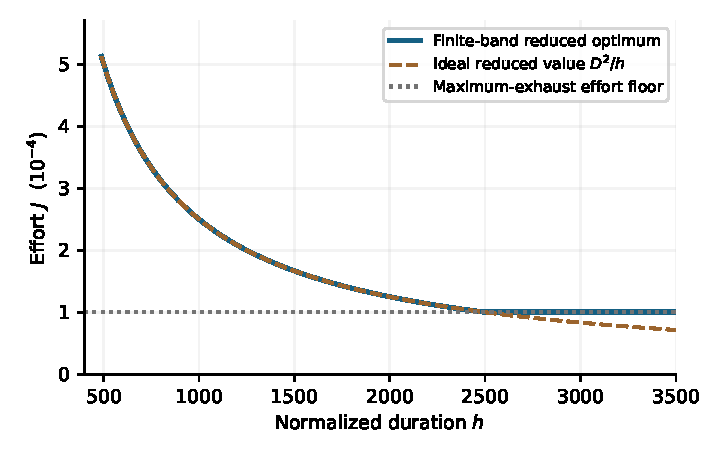
\includegraphics[width=\columnwidth]{figures/averaged_effort.pdf}
\caption{Minimum effort in the phase-free monotone circular model:
$D=0.5$, $\chi=0.01$, $\nu_-=10$, $\nu_+=50$.
The finite ceiling produces a long-duration fuel floor.}
\label{fig:spiral}
\end{figure}

Station phase adds a constraint. For constant acceleration the
accumulated angle is
\begin{equation}
 \Delta\theta=\frac h4(q_i^3+q_i^2q_f+q_iq_f^2+q_f^3).
\end{equation}
It is not a free output. On the maximum-exhaust plateau, let
$c=h-T_{\rm slow}$ and let $\Theta_b$ be the burn angle.
Placing coast at the initial and final radii gives exactly the range
\begin{equation}
 \Theta_b+c\min(q_i^3,q_f^3)
 \le\Delta\theta\le
 \Theta_b+c\max(q_i^3,q_f^3)
\end{equation}
at that minimum fuel, within the monotone approximation.
Outside this range phase costs additional effort or makes the chosen
duration infeasible. A fixed-phase ideal interior satisfies
$2q''=3\Lambda q^2$, rather than generally $q''=0$.

Neither reduced infeasibility nor its optimum is a full Kepler
certificate. Constant nonzero acceleration eventually makes
$|a_t|r^2$ large. For example, the earlier Earth illustration with
7000 km parking radius, chosen 900000 km SOI and useful
$P/m_0=540\,\mathrm{W/kg}$ gives an initial minimum powered
acceleration $0.00432\,\mathrm{m/s^2}$. Its slow-spiral diagnostic
already reaches $0.05$ near 67922 km from Earth's center.
The calculation is a validity warning for continuous slow spirals,
not a prediction of optimized Earth escape \cite{JPLParameters}.

\subsection{An exact feasible pair}
Exact analytic curves are useful independent tests of a controlled
Kepler solver \cite{PetropoulosSims2002}. In local units $\mu=1$, set
$0\le t\le10$ and
\begin{equation}
 \begin{gathered}
 r=1+0.03t^2,\qquad \theta=t/\sqrt r,\qquad \theta'=r^{-3/2},\\
 x=re_r,\quad v=0.06t\,e_r+r^{-1/2}e_\theta,\\
 u=0.06e_r+0.03t\,r^{-3/2}e_\theta.
 \end{gathered}
 \label{eq:exactescape}
\end{equation}
Direct differentiation gives $x''=-x/r^3+u$. It starts on the unit
circle, first reaches $r=4$ at $t=10$, and ends with
$\theta=5$, $v_r=0.6$, $v_t=0.5$, $E=0.055$.
The effort and a full-time acceleration enclosure are
\begin{equation}
 \begin{gathered}
 U=\frac{651}{16000}+\frac{\pi\sqrt3}{240}
 =0.0633599920529\ldots,\\
 0.06\le|u|\le\frac{\sqrt{181}}{150}<0.09.
 \end{gathered}
\end{equation}
With $\chi=0.9$, budget $0.08$, floor $0.8$ and band $[10,50]$,
$(\chi+U)/50<0.06$ and $\chi/10=0.09$.
Thus the curve is safe and band-feasible throughout, without relying
on sampling. It retains mass fraction $0.9342302020\ldots$.

Let $Q=\operatorname{diag}(1,-1)$. The reflected reversal
$x_c(t)=Qx(10-t)$, $v_c(t)=-Qv(10-t)$ and
$u_c(t)=Qu(10-t)$ preserves prograde angular momentum and arrives
at $(1,0,0,1)$. A unit station with initial phase $-10$ rendezvous
at this endpoint. The same magnitude enclosure proves band feasibility
for the same initial $\chi$, but the mass history is recomputed
forward: reversing position and velocity does not reverse fuel use.

\begin{figure}[tb]
\centering
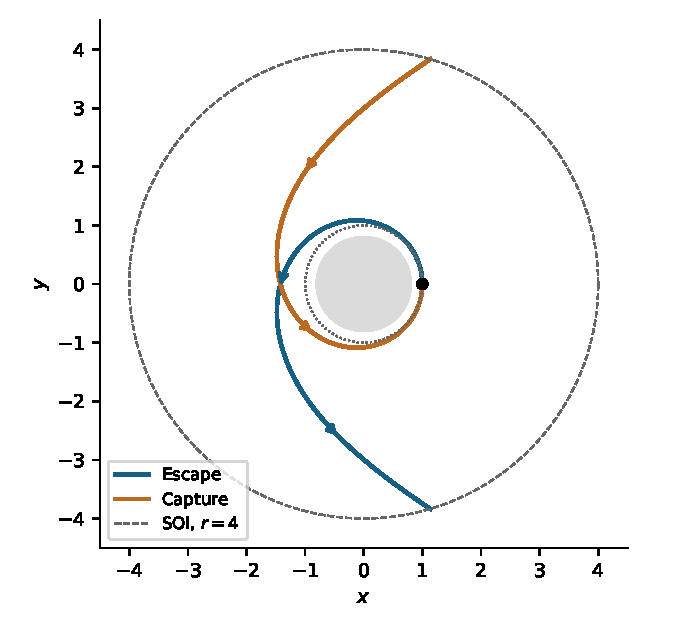
\includegraphics[width=\columnwidth]{figures/exact_escape_capture.pdf}
\caption{Exact escape and reflected capture examples. The station orbit
is dotted, the SOI is dashed, and $r<0.8$ is excluded.
These are separate feasible local trajectories.}
\label{fig:escape}
\end{figure}

For arbitrary endpoint energies in the annulus, define
$W_E=\sqrt{2E+2/\varepsilon}$. Since $|v|\le W_E$,
equation~\eqref{eq:work} gives $|W_E'|\le|u|$; also
$|j'|\le\sigma_S|u|$.
With $d_*=\max(|\Delta W_E|,|\Delta j|/\sigma_S)$, every
full-power/coast transfer satisfies
\begin{equation}
 J\ge
 \max\left\{\frac{d_*^2}{h},\
 \chi\left(e^{d_*/\nu_+}-1\right)\right\}.
 \label{eq:localbound}
\end{equation}
The second term follows from
$\int|u|dt\le\nu_+\log(1+J/\chi)$.
It remains valid for nonpositive $E$ whenever the endpoint states
are admissible.
For \eqref{eq:exactescape}, the energy part and feasible construction
give the symbolic same-endpoint bracket
\begin{equation}
 \frac{411-30\sqrt{174}}{1000}\le V_{\rm exact}\le
 \frac{651}{16000}+\frac{\pi\sqrt3}{240}.
 \label{eq:exactbracket}
\end{equation}
This establishes a feasible upper bound and a global lower bound in
the stated patch model; the constructed curve is not asserted stationary.

\section{What establishes optimality}
\label{sec:verification}
A useful planner needs a feasible trajectory and a reason to trust its
reported performance. These are separate outputs. A small shooting
residual indicates a stationary candidate; it does not establish a
minimum. Comparing feasible branches improves an upper bound, while
a lower bound must cover every admissible competitor.

\subsection{The smooth second variation}
For an exact ideal extremal strictly outside the floor, let
$z=(\delta r,\delta v)$ and $\xi=\delta u$ satisfy
$z'=Az+B\xi$, $z(0)=z(h)=0$.
The fixed-endpoint second variation is
\begin{equation}
 Q[\xi]=\int_0^h\left(2|\xi|^2-z^TC_s z\right)dt,
 \label{eq:second}
\end{equation}
with $C_s=\operatorname{diag}(K,0)$ and
\begin{equation}
 \begin{split}
 K={}&\frac3{R^5}
 [p_vr^T+rp_v^T+(p_v\cdot r)I]\\
 &-\frac{15(p_v\cdot r)}{R^7}rr^T,\qquad R=|r|.
 \end{split}
\end{equation}
Differentiating $Dg=-I/R^3+3rr^T/R^5$ and contracting its
derivative with $p_v$ gives the displayed $K$.
The sign and factor two follow by augmenting the minimized cost with
$\int p\cdot(s'-f)dt$. Coercivity
$Q\ge\gamma_Q\norm{\xi}_2^2$ with $\gamma_Q>0$ proves a strict
local minimum in the $L^2$ control topology; a negative direction on
the endpoint kernel rules it out.

Initialize the vertical Jacobi frame $X(0)=0$, $Y(0)=I$ and integrate
\begin{equation}
 \begin{pmatrix}X\\Y\end{pmatrix}'
 =\begin{pmatrix}A&D\\-C_s&-A^T\end{pmatrix}
 \begin{pmatrix}X\\Y\end{pmatrix}.
\end{equation}
Conjugate times are rank losses of $X(t)$ at $t>0$.
For this regular fully actuated acceleration problem, absence of
conjugate points on $(0,h]$ gives strict local minimality; a first
conjugate point strictly before $h$ produces a negative direction
on the longer interval \cite{Bonnard2007}.
Where $X$ is invertible, $S=YX^{-1}$ satisfies
\begin{equation}
 S'+A^TS+SA+SDS+C_s=0,
\end{equation}
and completing the square yields
$Q=[z^TSz]_0^h+2\int|\xi-B^TSz/2|^2dt$.
Initialize the frame, not an arbitrary $S(0)=0$.

Sampling $\det X$ cannot exclude conjugate points: even multiplicity
can leave its sign unchanged. The supplied synthetic accessory problem
$Q/2=\int_0^1(z''^2-600z^2)dt$ in two identical coordinates
has such a crossing at $t_c=0.955712066275\ldots$.
It also has the explicit negative direction $z=1-\cos(2\pi t)$.
The test verifies the diagnostic logic, not a particular orbital branch.
Engine switches, radial contacts and flybys need their own junction
terms in a second variation.

\subsection{Global effort lower bounds}
With floor $a>0$, gravity obeys $|g|\le g_m=a^{-2}$.
For the endpoint moments $d_r,d_v$ of \eqref{eq:free},
\begin{equation}
 L_v=\frac{\pos{|d_v|-g_mh}^2}{h},\qquad
 L_r=\frac{3\pos{|d_r|-g_mh^2/2}^2}{h^3}
 \label{eq:momentbounds}
\end{equation}
are lower bounds. They follow by integrating \eqref{eq:kepler}
and applying Cauchy--Schwarz.
A joint directional bound, for $\lambda=(\alpha,\beta)\ne0$, is
\begin{equation}
 \begin{gathered}
 L_\lambda=
 \frac{\pos{\lambda\cdot(d_r,d_v)-g_m\int_0^h|q(t)|dt}^2}
 {\lambda^TW_0\lambda},\\
 q(t)=(h-t)\alpha+\beta.
 \end{gathered}
\end{equation}
An upper enclosure of the convex norm integral preserves this bound.
Several directions may be evaluated cheaply at the actual query.

Energy and angular momentum supply additional bounds for competitors
with $J\le U$, where $U\ge0$ is any cutoff. Put
\begin{equation}
 \begin{split}
 c_0&=|v_0|^2+2/a-2/|r_0|,\\
 I_v(U)&=[h\sqrt U+\sqrt{h^2U+hc_0}]^2,\\
 R_U&=|r_0|+h|v_0|+g_mh^2/2+\sqrt{Uh^3/3}.
 \end{split}
\end{equation}
To see the first estimate, write $I=\int_0^h|v|^2dt$.
The work identity and Cauchy--Schwarz imply
$|v(t)|^2\le c_0+2\sqrt{UI}$, whence $I\le hc_0+2h\sqrt{UI}$.
Solving this quadratic inequality in $\sqrt I$ gives $I_v(U)$.
Double integration of acceleration and Cauchy--Schwarz give $R_U$.
Equation~\eqref{eq:work} gives
$\int|v|^2dt\le I_v(U)$ and $|r|\le R_U$, hence
\begin{equation}
 L_E=\frac{(\Delta E)^2}{I_v(U)},\qquad
 L_M=\frac{(\Delta j)^2}{hR_U^2}.
\end{equation}
Degenerate zero numerators and denominators are handled by continuity.
A globally valid combination is
\begin{equation}
 L=\max\{0,L_v,L_r,L_\lambda,
                  \min[U,\max(L_E,L_M)]\}\le V.
 \label{eq:globalL}
\end{equation}
The cutoff clipping covers trajectories with effort greater than $U$.
An actually feasible trajectory of effort at most $U$ additionally
establishes $V\le U$ and suboptimality at most $U-L$.
Ideal lower bounds also apply to the bounded engine at the same
endpoints; its upper bound needs a band-feasible witness.

\subsection{A global certificate near a low-effort path}
Let $(\bar r,\bar v,\bar u)$ be an endpoint-exact feasible ideal
reference of effort $U$ and $p$ any continuous piecewise differentiable
multiplier. Define residuals
\begin{equation}
 e_u=2\bar u-p_v,\quad
 e_r=p_r'+Dg(\bar r)^Tp_v,\quad e_v=p_v'+p_r.
\end{equation}
For a competitor, write $\delta u=u-\bar u$,
$\delta r=r-\bar r$, $\delta v=v-\bar v$ and
$R_g=g(r)-g(\bar r)-Dg(\bar r)\delta r$.
Integration by parts gives the exact difference
\begin{equation}
 \begin{split}
 J-U={}&\norm{\delta u}_2^2+\int e_u\cdot\delta u\,dt\\
 &-\int(e_r\cdot\delta r+e_v\cdot\delta v+p_v\cdot R_g)dt.
 \end{split}
 \label{eq:gapidentity}
\end{equation}
Endpoint error would add a boundary term; it cannot be ignored.

Suppose $|\bar r|\ge b>a$, choose $0<d<b$ and put
$\ell=b-d$, $\omega=\sqrt{2/\ell^3}$.
Before a first exit from $|\delta r|<d$,
\begin{equation}
 |\delta r(t)|\le k_r(t)\norm{\delta u}_{2,[0,t]},\quad
 |\delta v(t)|\le k_v(t)\norm{\delta u}_{2,[0,t]},
\end{equation}
where
\begin{equation}
 k_r(t)^2=\int_0^t\frac{\sinh^2(\omega s)}{\omega^2}ds,\quad
 k_v(t)^2=\int_0^t\cosh^2(\omega s)ds.
\end{equation}
Every competitor with $J\le U$ has
$\norm{\delta u}_2\le2\sqrt U$. Thus
\begin{equation}
 2\sqrt U\,k_r(h)<d
 \label{eq:containment}
\end{equation}
prevents a first exit and covers all cheaper competitors.

Let $A_r=\int_0^h k_r^2dt$, $A_v=\int_0^h k_v^2dt$,
$P_v\ge\sup|p_v|$ and
\begin{equation}
 \begin{gathered}
 \gamma=1-\frac{3P_v}{\ell^4}A_r,\\
 \eta=\norm{e_u}_2+\sqrt{A_r}\norm{e_r}_2+
                    \sqrt{A_v}\norm{e_v}_2.
 \end{gathered}
\end{equation}
The sharp bound is $\norm{D^2g(x)[z,z]}\le6|z|^2/|x|^4$.
Indeed
\[
D^2g(x)[z,z]=\frac{6(x\cdot z)z+3|z|^2x}{|x|^5}
             -\frac{15(x\cdot z)^2x}{|x|^7}.
\]
For $|z|=1$ and $c=\hat x\cdot z$, its squared norm is
$9(1-2c^2+5c^4)/|x|^8\le36/|x|^8$, with equality radially.
Taylor's factor $1/2$ therefore gives $|R_g|\le3|\delta r|^2/\ell^4$.
This tightens the earlier factor 12 in $\gamma$ to 3 and implies $J-U\ge\gamma s^2-\eta s$ with $s=\norm{\delta u}_2$.
If \eqref{eq:containment} holds and $\gamma>0$,
\begin{equation}
 \boxed{\max(0,U-\eta^2/(4\gamma))\le V\le U.}
 \label{eq:tubegap}
\end{equation}
For an exact extremal $\eta=0$ proves uniqueness of the global
minimum, up to equality of controls almost everywhere. Numerical
use requires validated enclosures of the reference, residual norms
and constants. Sampled minima with padding do not supply that proof.

The earlier nonzero-effort fixture near $J=0.0032$ gives a small
double-precision estimate of the gap in \eqref{eq:tubegap}; it remains
an estimate, not a machine-verified certificate.
For difficult cells a verification function satisfying
$W_t+W_r\cdot v+W_v\cdot g-|W_v|^2/4\ge0$
throughout every possible cheaper trajectory yields another lower
bound by integration. A sampled residual mesh is insufficient.

\subsection{The atlas decision}
Store model, winding and active-set labels with every branch, together
with endpoint residuals, feasible reconstruction, effort enclosure,
and the domain and provenance of each optimality claim.
A point proof does not certify the surrounding interpolation cell.
Uniform continuation, constraint bounds and second-variation or
global-gap bounds must cover that cell.

At a query, combine valid lower bounds by their maximum and feasible
upper bounds by their minimum. Return infeasible if $L>\kappa$,
feasible if $U\le\kappa$, and unresolved otherwise.
A failed sufficient test is unresolved. An extra revolution alone is
not grounds for rejection: a circular coast over $4\pi$ is a two-turn
global zero-effort minimum for its own endpoints.

\section{Local rendezvous and pursuit}
\label{sec:cw}
The same effort resource gives an exact local linear problem. In a frame
rotating with a reference circle, use
$s=(x,y,\dot x,\dot y)$ with unit mean motion. The planar
Clohessy--Wiltshire system \cite{ClohessyWiltshire1960} is
\begin{equation}
 \begin{gathered}
 s'=As+Bu,\\
 A=\begin{pmatrix}
 0&0&1&0\\0&0&0&1\\3&0&0&2\\0&0&-2&0
 \end{pmatrix},\quad B=\begin{pmatrix}0&0\\0&0\\1&0\\0&1\end{pmatrix}.
 \end{gathered}
\end{equation}
Let $\Phi(t)=e^{At}$ and
$W(h)=\int_0^h\Phi(t)BB^T\Phi(t)^Tdt$.
Controllability makes $W$ positive definite for every $h>0$.
For $y_f=s_f-\Phi(h)s_0$,
\begin{equation}
 J^*=y_f^TW^{-1}y_f,\qquad
 u^*(t)=B^T\Phi(h-t)^TW^{-1}y_f.
 \label{eq:cwcost}
\end{equation}
The reachable set at budget $b$ is the ellipsoid $J^*\le b$.
Projecting to position uses the upper-left $2\times2$ block of $W$.
The center is the unforced CW trajectory. Appendix~\ref{app:interval} gives the trigonometric transition and
Gramian entries. Their Taylor series supply the small-time limit;
a scaled Cholesky solve avoids explicit inversion.

\subsection{The ideal rendezvous game}
Let $z=s_E-s_P$, with reserves $b_E,b_P$. Set
\begin{equation}
 \begin{gathered}
 K(t)=\Phi(-t)B,\qquad M(h)=\int_0^hK(t)K(t)^Tdt,\\
 C(h)=z_0^TM(h)^{-1}z_0.
 \end{gathered}
\end{equation}
For $z_0\ne0$, $C$ decreases continuously and strictly from infinity
to zero. Its derivative is
$C'(h)=-|K(h)^TM(h)^{-1}z_0|^2$.
The strict monotonicity follows from controllability on every interval;
the large-time zero limit follows from the explicit CW Gramian.

\begin{theorem}[Ideal CW rendezvous]
With unrestricted $L^2$ controls, no further state constraints and
instantaneous observation of the evader's control by the pursuer,
the minimum guaranteed time to full-state rendezvous is the unique
$H>0$ solving
\begin{equation}
 C(H)=(\sqrt{b_P}-\sqrt{b_E})^2
\end{equation}
when $b_P>b_E$. If $b_P\le b_E$ and $z_0\ne0$, the value is
infinite. At $z_0=0$ it is zero.
\end{theorem}
For the upper bound use $a_H(t)=K(t)^TM(H)^{-1}z_0$ and
$u_P=u_E+a_H$. The relative endpoint is exactly zero, and
Minkowski's inequality gives
$\norm{u_P}_2\le\sqrt{b_E}+\sqrt{C(H)}=\sqrt{b_P}$.
The opposing strategy and parity argument appear in
Appendix~\ref{app:game}; the result uses the integral-constraint
game framework \cite{Ibragimov2011}.
Full-state rendezvous is not position-only interception or capture
within a finite radius.

\subsection{A sufficient nonlinear extension}
For rotating position $q$, the exact Kepler equation is
\begin{equation}
 q''+2\rot q'=\operatorname{diag}(3,0)q+u+N(q),
\end{equation}
where
$N(q)=-(e_1+q)/|e_1+q|^3+e_1-\operatorname{diag}(2,-1)q$.
On $|q|\le\epsilon<1$,
\begin{equation}
 |N(q)|\le N_\epsilon=\frac{3\epsilon^2}{(1-\epsilon)^4},\quad
 \operatorname{Lip}(N)\le L_\epsilon=
                   \frac{6\epsilon}{(1-\epsilon)^4}.
\end{equation}
These finite-domain inequalities follow from
$\norm{D^2g(x)[u,v]}\le6|u||v|/|x|^4$ and Taylor's formula.

Use
$u_P=u_E+a_h+N(q_E)-N(q_P)$. It cancels the nonlinear relative
remainder, giving exactly the CW correction trajectory $z_h$.
If both paths remain in the ball, then
\begin{equation}
 \sqrt{b_P}\ge\sqrt{b_E}+\sqrt{C(h)}
       +L_\epsilon\left(\int_0^h|\Pi z_h(t)|^2dt\right)^{1/2}
 \label{eq:cwcert}
\end{equation}
guarantees rendezvous by $h$, where $\Pi=(I,0)$.
Appendix~\ref{app:tube} gives an explicit first-exit tube bound, and Appendix~\ref{app:inertial} gives an inertial half-space alternative for wider separations.
The same tube inflates a single-ship reachable ellipsoid to budget
$(\sqrt b+N_\epsilon\sqrt h)^2$, giving an outer reachability bound.

These capture results concern the ideal engine. A restricted ship's
reachable set is contained in the ideal set, but restricting both
players need not preserve the ideal winner. A bounded-engine capture
guarantee requires admissibility against every permitted opponent.
Checking one saddle trajectory or clipping the compensating control
does not establish that guarantee.

\section{Interception and deadline-fuel games}
\label{sec:interception}
This section restores position-only interception, needed for contact or
salvage races. Boarding instead requires velocity matching. All closed
forms here use the ideal engine and instantaneous nonanticipative response;
they are not finite-band game values. Write $r=x_E-x_P$, $w=v_E-v_P$,
and take capture to mean $|r|\le R$. Resources in this section may be
physical, with $g=-\mu x/|x|^3$, or consistently normalized.

\subsection{The four problems and verification}
Let $z=(x_P,v_P,x_E,v_E,b_P,b_E)$ and
\[
 \mathcal D U=U_{x_P}\cdot v_P+U_{v_P}\cdot g(x_P)
              +U_{x_E}\cdot v_E+U_{v_E}\cdot g(x_E).
\]
The Isaacs operator for pursuer running cost $\ell|a_P|^2$ is
\begin{equation}
\begin{split}
\mathcal H_\ell U={}&\mathcal D U+
 \inf_{a_P}\{U_{v_P}\cdot a_P+(\ell-U_{b_P})|a_P|^2\}\\
 &+\sup_{a_E}\{U_{v_E}\cdot a_E-U_{b_E}|a_E|^2\}.
\end{split}
\end{equation}
At a zero resource face the corresponding control is zero. Where
$c_P=\ell-U_{b_P}>0$ and $c_E=U_{b_E}>0$, this becomes
\begin{equation}
 \begin{gathered}
 \mathcal H_\ell U=\mathcal D U-
 \frac{|U_{v_P}|^2}{4c_P}+\frac{|U_{v_E}|^2}{4c_E},\\
 a_P^*=-\frac{U_{v_P}}{2c_P},\qquad a_E^*=\frac{U_{v_E}}{2c_E}.
 \end{gathered}
\end{equation}
Zero or wrong-sign coefficients require evaluating the original extrema,
including infinite values, rather than dividing by zero.
Problems A1 and B1 minimize guaranteed interception time in free space
and Kepler gravity, respectively: $1+\mathcal H_0V=0$, $V=0$ on capture.
Problems A2 and B2 minimize worst-case pursuer effort to capture within
remaining time $s$: $W_s=\mathcal H_1W$, with $W=0$ on capture and
$W(0,z)=+\infty$ outside capture. Failure to capture by the deadline costs
$+\infty$; the budget state remains a hard constraint.

\begin{proposition}[Classical verification]
Suppose a nonnegative differentiable solution satisfies the stated PDE,
target and resource boundary conditions. Suppose its selectors generate
well-posed admissible responses throughout the relevant domain. For time,
the pursuer selector guarantees capture and the evader selector gives the
opposing time bound. For deadline effort, assume additionally that the
pursuer selector guarantees capture before the deadline. Then the solution
is the respective value, provided the boundary limits used at capture
and exhaustion exist.
\end{proposition}
Indeed, along the time pursuer selector, $dV/dt\le-1$ against every
evader, whereas along the evader selector $dV/dt\ge-1$ against every
pursuer. Integrate to capture; nonnegativity supplies the time upper
bound. For remaining time $s'= -1$, along the deadline pursuer selector,
$dW/dt+|a_P|^2\le0$, and along the evader selector the inequality reverses.
Integration gives the opposing effort bounds; noncapture has infinite
cost. Localization and boundary limits are essential. Nonsmooth values
require viscosity and comparison hypotheses \cite{EvansSouganidis1984};
this verification statement does not assert existence for an unrestricted
singular orbital domain.

\subsection{Closed forms and distinctions}
Against a ballistic evader in free space, set
$d(h)=(1-R/|r+hw|)_+(r+hw)$, with $d=0$ at zero separation. The exact
prescribed-time interception effort and control are
\begin{equation}
 c(h)=\frac{3|d(h)|^2}{h^3},\qquad a_P(t)=\frac{3(h-t)}{h^3}d(h).
\end{equation}
These follow by projecting the required position onto the capture ball
and using the single moment $\int_0^h(h-t)a_Pdt=d$. Deadline fuel is
$\inf_{0<h\le T}c(h)$ and earliest interception is
$\inf\{h:c(h)\le b_P\}$. In particular, if $c(h)>b_P$ for every
$0<h\le T$, coasting is a zero-fuel evader win, even when fuel is available.

For active interception with $w=0$, $D=|r|-R>0$, $b_P>b_E$ and
$b_P\ge4b_E$, the exact guaranteed time is
\begin{equation}
 H_I=\left[\frac{3D^2}{(\sqrt{b_P}-\sqrt{b_E})^2}\right]^{1/3}.
\end{equation}
Put $k=\sqrt{b_E}/(\sqrt{b_P}-\sqrt{b_E})\le1$ and
$a_0(t)=3D(1-t/H_I)r/(H_I^2|r|)$. The response $a_P=a_E+a_0$
gives the upper bound by Minkowski. The opponent $a_E=ka_0$ prevents an
earlier hit: at $t=sH_I< H_I$ any pursuer needs at least
$C s^{-3}[1+kf(s)]^2$, where $C=3D^2/H_I^3$ and
$f(s)=(3s^2-s^3)/2$. This exceeds $(1+k)^2C=b_P$ because
\[
\begin{split}
1+kf(s)-(1+k)s^{3/2}
={}&(1-k)(1-s^{3/2})\\
 &+k[1+f(s)-2s^{3/2}]>0;
\end{split}
\]
use $f(s)\ge s^3$. For point capture ($R=0$), full-state boarding takes
$4^{1/3}H_I$ under these same hypotheses.

For a prescribed exact endpoint at time $h$, let
\begin{equation}
 \begin{gathered}
 C_I=3|r+hw|^2/h^3,\\
 C_J=12|r|^2/h^3+12r\cdot w/h^2+4|w|^2/h.
 \end{gathered}
\end{equation}
The endpoint minimax pursuer effort is
\begin{equation}
 M_{I,J}(h)=(\sqrt{b_E}+\sqrt{C_{I,J}(h)})^2.
\end{equation}
The copying response gives the upper bound. Choosing the evader control
proportional to the minimum-norm endpoint correction gives the lower
bound by orthogonal projection onto the endpoint moment constraints.
This is an exact-time endpoint result. Minimizing it over deadlines gives
a sufficient first-hit bound, not automatically the first-hit value.
For perpetual avoidance of exact rendezvous at a nonzero phase state,
$b_E\ge b_P$ gives least worst-case evader expenditure
$F^J_\infty=b_P$. The parity feedback in Appendix~\ref{app:game} attains
the upper bound; a smaller uniform expenditure cap would give the
pursuer a strictly positive resource gap and finite-time rendezvous.

\paragraph{Nonattainment matters.}
Strict position-only escape can have an infimum without a minimizing
control. An exhausted stationary pursuer at the origin and an evader
coasting from $(-L,R)$ with velocity $(u,0)$ meet the capture boundary
at $L/u$. Any arbitrarily small positive transverse thrust before that
time avoids it forever, at cost tending to zero; zero thrust loses.
There are also positive unattained infima. In one dimension take point
capture, separation $L>0$, closing velocity $-u<0$, and an exhausted
pursuer. The critical effort is $4u^3/(9L)$: the endpoint lower bound
$3(ut-L)^2/t^3$ is largest at $t=3L/u$. Equality forces contact there.
The safe profiles $r(t)=\delta+(L-\delta)(1-t/t_\delta)^3$ for
$0\le t\le t_\delta=3(L-\delta)/u$, followed by rest at $\delta>0$,
approach that cost as $\delta\downarrow0$ without attaining it.

\subsection{Five-state reduction and scaling}
In isotropic free space a value depends only on
$(\rho_G,\xi_G,\omega_G,b_P,b_E)=(|r|^2,r\cdot w,|w|^2,b_P,b_E)$,
where $\xi_G^2\le\rho_G\omega_G$. The drift is
$2\xi_G U_{\rho_G}+\omega_G U_{\xi_G}$ and
\begin{equation}
 |U_w|^2=\rho_G U_{\xi_G}^2+4\xi_G U_{\xi_G}U_{\omega_G}
                      +4\omega_G U_{\omega_G}^2.
\end{equation}
Both controlled velocity gradients have this squared norm. These chain
rules reduce the free-space Isaacs equation to five states in $d=2$ or
$3$. Under $t\mapsto\alpha t$, $r\mapsto\beta r$,
$w\mapsto(\beta/\alpha)w$, resources scale as $\beta^2/\alpha^3$.
Time values scale by $\alpha$, and deadline-fuel values by
$\beta^2/\alpha^3$, with radius and deadline scaled as well. Scaling
every strategy and opponent proves the rule for values, not only paths.

Finally, restore dimensional mean motion $n$ in the CW matrices. As
$n\to0$, $\Phi_n$ and $W_n$ converge to the double-integrator matrices.
Theorem~1 therefore reduces to the free-space cubic
\begin{equation}
 (\sqrt{b_P}-\sqrt{b_E})^2H^3-4|w|^2H^2
       -12r\cdot w H-12|r|^2=0.
\end{equation}
One takes this physical limit before setting the normalized mean motion
to one.


\section{Heliocentric checks and worked bounded cases}
\label{sec:helio}
Use $R_0=149597870700$ m and
$\mu_\odot=1.32712440018\,10^{20}$ $\mathrm{m^3/s^2}$.
Then $T_0=58.13244087$ days, $V_0=29.78469183$ km/s and
$J_0=176.6257101$ $\mathrm{m^2/s^3}$.

\subsection{Revisiting the Jupiter-class candidates of the transfer article}
The ideal engine of \cite{OriginalKepler} has $P=1$ GW, $m_0=3\,10^6$ kg and
$m_d=10^6$ kg: $\chi=3.774459936$ and $\kappa=7.548919872$.
The public atlas of \cite{OriginalKepler} supplies warm starts, not
certified trajectories. We independently integrate the normalized Cartesian state,
effort adjoints and effort quadrature, and solve four endpoint equations
plus $J=\kappa$. This avoids relying on the repository viewer's radius
and angle acceptance tolerances. The geometries below reproduce the
short-arc table and the two illustrated solar-pass families of the
transfer article, allowing for its rounded figure labels.

\begin{center}\small
\begin{tabular}{rrrrr}\toprule
$\rho,\Theta$&days&$r_{\min}$ AU&$v_{e,\min}$&$v_{e,\max}$\\\midrule
$5.2,80^\circ$&170.034&1.0000&40.60&2984.8\\
$5.0,273.1^\circ$&206.560&0.16993&42.35&13001.0\\
$5.2,385.2^\circ$&214.236&0.000273&4.85&1203.5\\\bottomrule
\end{tabular}\end{center}
Exhaust speeds are in km/s. All three paths fail the band. The first two
have numerical radius minima above 0.1 AU; the last also fails the floor.
Scaled endpoint residuals are below $4\,10^{-13}$ for the first two and
$10^{-8}$ for the last. The long-arc solve uses polar equations and
analytic shooting sensitivities to preserve its winding; a radial-velocity
root refines its narrow perihelion, which uniform samples alone miss.


We also reconstruct all 73 rows of that article's $5.2$ AU final-polar-angle
table, $\Theta=0^\circ,5^\circ,\ldots,360^\circ$, by independent continuation.
Every row violates the exhaust band. Their reconstructed times range from
$169.7643$ to $220.4991$ days (the $0^\circ$ row lies outside the abbreviated
170--215 day range). Scaled endpoint residuals are below $4.8\,10^{-11}$.
The radial audit locates turning points rather than only testing a time grid:
\begin{center}\small
\begin{tabular}{lrr}\toprule
Final-angle rows&Band rejected&Floor rejected\\\midrule
$0^\circ$--$300^\circ$ (61 rows)&61&0\\
$305^\circ$--$360^\circ$ (12 rows)&12&12\\\bottomrule
\end{tabular}\end{center}
For example, the numerical minimum radius is $0.1011887$ AU at $300^\circ$
and $0.090577$ AU at $305^\circ$. Thus none of these 73 candidates, nor
either illustrated solar-pass candidate, survives both operational checks.

The audit evaluates $v_e=V_0(\chi+I)/|u|$ and the radius on a dense
40001-point reconstruction, with continuous refinement of the long-arc
perihelion and exhaust extrema. Each reported band rejection has a large
violation on a continuous powered interval, so it does not depend on
interpreting an isolated zero-thrust sample. Clipping a failed trajectory
to the band does not repair its endpoint. The input seeds and normalized initial covectors are provided as
supplementary material.

\subsection{A local certificate demonstration: a 2.9-day solar hop}
This example raises the heliocentric radius from $1$ to $1.001$ AU
in $2.90663$ days and ends on a slightly eccentric orbit. Its purpose
is to demonstrate an explicit feasible path together with global effort
and time bounds on a small, fully checkable case.
For this auditable local example, keep $P=1$ GW and $m_0=3\,10^6$ kg,
but choose the smaller resource $\kappa=0.0320066666667$. Begin on the
unit circular orbit and let $c=0.4$, $H=0.05$. Define a physical
heliocentric path through its normalized polar coordinates:
\begin{equation}
 \begin{gathered}
 r(t)=1+ct^2,\qquad \theta(t)=\frac{t}{\sqrt{1+ct^2}},\\
 v_r=2ct,\qquad v_\theta=r^{-1/2}.
 \end{gathered}
\end{equation}
Since $\theta'=r^{-3/2}$, exact substitution into the Kepler equations
gives $u_r=2c$ and $u_\theta=ct/r^{3/2}$. Thus this is a continuously
powered exact path with $r\ge1$ AU, not a patched approximation. Its
endpoint defines the target: take the unforced Kepler orbit through
$(r(H),\theta(H),v_r(H),v_\theta(H))$ at epoch $H$. The arrival orbit is
slightly eccentric.
Coasting along that orbit is admissible on the short horizon used below.
The same backward comparison used below bounds its separation from the
unit circle by $0.0031$ on $[0,H]$, so the target orbit also clears the floor.

The effort and a convenient elementary upper bound are
\begin{equation}
\begin{split}
 J&=4c^2H+c^2\int_0^H\frac{t^2}{(1+ct^2)^3}dt\\
  &=0.0320066546838,\\
 U&=4c^2H+c^2H^3/3=0.0320066666667=\kappa.
\end{split}
\end{equation}
Mass accounting gives $m_d=2974774.5061$ kg from the budget and an actual
propellant expenditure $25225.4845$ kg for this witness. The burn satisfies
$0.8\le|u|\le\sqrt{0.64+0.16H^2}$ and $\chi\le w\le\chi+U$.
Consequently its full-power exhaust remains between $140.4825$ and
$141.7181$ km/s, strictly within the required band, throughout the path.

Here is a global, conservative lower-bound calculation, which also
brackets the minimum time instead of assigning optimality to this shaped
path. Compare every competitor of effort at most $U$ with the unit
circular coast. In a position tube of radius $d=0.1$, the gravity
Lipschitz constant is $K=2/0.9^3$, $\omega=\sqrt K$.
Variation of constants and Cauchy--Schwarz give
\begin{equation}
 |\delta r(t)|\le k_r(t)\sqrt J,\qquad
 |\delta v(t)|\le k_v(t)\sqrt J,
\end{equation}
where $k_r,k_v$ are those in Section~\ref{sec:verification}. Since
$\sqrt U k_r(H)<0.0012<0.1$, the first-exit argument validates this tube
for every cheaper competitor, irrespective of its thrust direction.
The target endpoint has $|\delta v(H)|>0.0399$ and
$k_v(H)^2\le H\cosh^2(\omega H)<1.007H$. Therefore
\begin{equation}
 0.0316=L\le F^*(0,H)\le U=0.0320066666667.
\end{equation}
The clipping argument from \eqref{eq:globalL} covers more expensive
competitors as well. These same bounds hold for the restricted engine,
because its witness passes the band and its competitors are a subset of
the ideal ones.

For an earlier arrival at $h_-=0.049$, compare the ballistic target to
the unit coast backward from $H$. At $H$, $|\delta r|<0.00101$ and
$|\delta v|<0.041$. Over $H-h_-=0.001$, the comparison inequalities
give $|\delta r|<0.0011$ and a change in $\delta v$ of less than
$K(0.0011)(0.001)<0.0000031$. Hence every affordable earlier competitor
would need
\begin{equation}
 J\ge\frac{(0.0399-0.0000031)^2}{1.007(0.049)}
   >0.0322591>\kappa,
\end{equation}
a contradiction. Coast extension and the monotone value then exclude
all still earlier arrivals. Thus the resource-to-time-to-fuel calculation is
\begin{equation}
 \boxed{\begin{gathered}0.049<h^*(\kappa)\le0.05,\\
 2.84848<T^*\le2.90663\ {\rm days}.\end{gathered}}
\end{equation}
The stated fuel is that of the witness path; the optimal duration lies
somewhere in this interval. The conservative decimal
inequalities can be checked by rational Taylor enclosures; a supplementary
checker does so for the bounds used in the time bracket.


\subsection{A certified 70-day Earth--Mars witness}
\label{sec:marswitness}
For an interplanetary performance point, return to $P=1$ GW,
$m_0=3\,10^6$ kg and $m_d=10^6$ kg, hence
$\kappa=7.548919872$. Use coplanar circular planetary orbits at
$1$ and $R_M=1.524$ AU in the solar two-body model. The following
explicit path gives full position-and-velocity rendezvous in exactly
70 days, with useful jet power fixed at 1 GW throughout. The exhaust
schedule is variable and satisfies the two-sided $50$--$250$ km/s band.

Let $H=70(86400)/T_0$ and $q=0.51011006$, with the decimal exact.
Set $c_q=(1-q^2)/(1+q^2)$ and $s_q=2q/(1+q^2)$. The endpoint states are
\begin{equation}
\begin{gathered}
 r_0=(1,0),\qquad v_0=(0,1),\\
 r_8=R_M(c_q,s_q),\qquad
 v_8=R_M^{-1/2}(-s_q,c_q).
\end{gathered}
\end{equation}
The circular target passes through this endpoint at $H$. Thus its
initial phase is $2\arctan q-H/R_M^{3/2}$, approximately
$17.3820101^\circ$ ahead of Earth; arrival longitude is approximately
$54.0531714^\circ$. Planetary
escape, capture, parking-orbit costs and departure waiting time are
outside this heliocentric model.

\begin{table*}[t]
\centering\small
\caption{Exact rational interior knots of the 70-day witness. Entries
are exact defining decimals. Positions and velocities use the solar normalized units.
Endpoint knots are $t_0=0$, $t_8=H$ and the analytic states in the text.}
\label{tab:marsknots}
\begin{tabular}{rrrrrr}\toprule
$j$ & $t_j/H$ & $r_{jx}$ & $r_{jy}$ & $v_{jx}$ & $v_{jy}$\\\midrule
1 & 0.137169299389 & 1.001350238628 & 0.168727459300 & 0.017525621592 & 1.046344765303\\
2 & 0.274338598779 & 1.006411818893 & 0.346210491047 & 0.046245191438 & 1.105077859977\\
3 & 0.411507898168 & 1.017566072445 & 0.534820743099 & 0.091838207401 & 1.182668462417\\
4 & 0.548677197557 & 1.037723200329 & 0.738442255030 & 0.154970973170 & 1.288219089473\\
5 & 0.661507898168 & 1.043707872696 & 0.902107682569 & -0.064178195495 & 1.117609239693\\
6 & 0.774338598779 & 1.020891188142 & 1.041194789559 & -0.269833623616 & 0.926300052106\\
7 & 0.887169299389 & 0.970819319098 & 1.152810168550 & -0.465866897104 & 0.712855383845\\
\bottomrule\end{tabular}
\end{table*}

On interval $j=0,\ldots,7$, put $\Delta_j=t_{j+1}-t_j$,
$s=(t-t_j)/\Delta_j$ and use cubic Hermite interpolation:
\begin{equation}
\begin{split}
 r(t)={}&(2s^3-3s^2+1)r_j
       +(s^3-2s^2+s)\Delta_j v_j\\
 &+(-2s^3+3s^2)r_{j+1}
       +(s^3-s^2)\Delta_j v_{j+1}.
\end{split}
\label{eq:marshermite}
\end{equation}
Table~\ref{tab:marsknots} and the analytic endpoints specify the whole
path. Define its control and mass by
\begin{equation}
\begin{gathered}
 u=r''+r/|r|^3,\qquad I(t)=\int_0^t|u|^2\,ds,\\
 m(t)=\frac{m_0\chi}{\chi+I(t)},\qquad
 v_e(t)=V_0\frac{\chi+I(t)}{|u(t)|}.
\end{gathered}
\end{equation}
The position and velocity are continuous and the endpoint conditions
hold exactly by construction. Acceleration may jump at knots; the
model imposes no thrust-slew constraint. Each one-sided control value
passes the band. The resulting mass, thrust and exhaust obey the
constant-power equations exactly almost everywhere.

A whole-interval enclosure gives
\begin{equation}
\begin{gathered}
 2.5212<J<2.5307< U_M=2.6<\kappa,\\
 99<v_e(t)<102\ {\rm km/s},\qquad |r(t)|>0.999\ {\rm AU},\\
 1.2014\,10^6<m_0-m(H)<1.2041\,10^6\ {\rm kg}.
\end{gathered}
\end{equation}
In particular, the spacecraft retains over $1.7959\,10^6$ kg, above
the dry-mass floor. Consequently, for this target phase,
\begin{equation}
 \boxed{F_{\rm band}^*(0,H)\le U_M=2.6,\qquad T_{\rm band}^*(\kappa)\le70\ {\rm days}.}
\end{equation}
This is an unoptimized upper bound on the minimum time. Comparing it
with an ideal-engine optimum for the same endpoints, to measure the
time cost of the band, is left for future work.

Here is a reproducible enclosure prescription. Form the Hermite cubic
coefficients from the defining decimals, using outward interval arithmetic
at 60 significant decimal digits, including the square roots in $T_0$,
$V_0$ and the terminal velocity. Subdivide each of the eight local
$s$ intervals into 128 equal parts. Horner evaluation encloses $r$ and
$r''$; square, sum and take an outward square root to bound $|r|$,
then enclose $u$ and $|u|^2$. Multiplying each latter enclosure by its
time width gives lower and upper Riemann bounds for $I$. For the
exhaust check on a subinterval, use the cumulative lower bound at its
start and cumulative upper bound at its end. This monotonic enclosure
covers every time within it. The resulting bounds imply the displayed
coarse inequalities. A standalone supplementary checker implements
this recipe; a separate floating-point quadrature and dynamics
integration provide independent numerical cross-checks.

\section{Computation and reproducible evidence}
\label{sec:computation}
\subsection{Offline branches, online decisions}
The intended runtime is a few milliseconds, so full boundary-value
solves belong offline. Continue endpoint-exact branches over geometry,
time, vehicle and active-set coordinates; retain competing windings
and encounter sequences. Audit engine and radial feasibility, compute
variational data, and attach the strongest verified performance bounds
available. A surrogate must preserve its branch domain and an error
bound; interpolated controls need endpoint correction.

At runtime, normalize the actual vehicle and endpoints, retrieve
candidate branches, and propagate actual mass through the route.
Use \eqref{eq:pointgrad} or \eqref{eq:soichart} to optimize stored
phase couplings, evaluate lower and feasible upper bounds, and search
duration with a maintained bracket. Interior stationary events disappear
from the outer first variation, but their feasibility and optimality
status remain part of the route status.
An unresolved budget test calls for refinement, not an infeasibility label.

The following distinctions are useful output fields:
\begin{center}
\small
\begin{tabular}{@{}p{0.29\columnwidth}p{0.65\columnwidth}@{}}
\toprule
Status & Evidence required\\\midrule
Feasible & Endpoint, dynamics, resource and path checks\\
Stationary & Correct PMP and all junction residuals\\
Local minimum & Valid second-order sufficiency\\
Bounded gap & Valid global $L$ and feasible $U$\\
Global minimum & Matching bounds or a global proof\\
\bottomrule
\end{tabular}
\end{center}
These fields are not inferred from a solver's successful return code.
Normal PMP conditions alone also do not enumerate possible abnormal
extremals or prove ordinary-control attainment in a nonconvex on/off
problem.

\subsection{Three consistency checks}
The following reproducible identities check the interfaces between formulas.

\paragraph{Timing and control gain.}
Circular-endpoint shooting checks both
$F_h=-|u_f|^2$ and $F_d=(\omega-1)\mathcal L$ against its endpoint
data. Substituting $p_v=2u$, $C=1$ in the bounded selector recovers
$\mathcal G=|u|^2$ whenever the band is inactive. The exact-rational
nonconvexity certificate is rerun separately; it proves the leading
Jensen-gap sign, not global optimality of a selected finite perturbation.

\paragraph{One physical mass, several local units.}
Take an artificial accounting example with $m_0=1000$ kg, $P=10^6$ W,
and two physical efforts $j_1=20$, $j_2=40$ in
$\mathrm{m^2/s^3}$. Equation~\eqref{eq:route_mass} gives
$m_f=970.8737864078$ kg.
Assigning effort scales $J_{0,1}=2$ and $J_{0,2}=5$ changes the
normalized efforts to $10$ and $8$, but gives the same mass when each
entry $\chi$ is computed from the actual entry mass. Incorrectly
resetting the second leg to $m_0$ gives $980.3921568627$ kg.
With the second power changed to $2\,10^6$ W, the correct final mass
is also $980.3921568627$ kg: the equality is coincidental and illustrates
why power belongs in the accounting. These are algebraic examples,
not trajectories.

\paragraph{SOI action and covectors.}
Deterministic randomized transverse crossings verify that
\eqref{eq:zeta} makes all four chart derivatives in
\eqref{eq:soichart} vanish, that the relative Hamiltonian matches,
and that the state saltation matrix produces the same covector jump.
Independent scale-pairing checks verify \eqref{eq:covscale}.
Both entry and exit signs are exercised. These are interface identities;
they do not demonstrate an optimized complete route.

\subsection{Trajectory test cases}
The reduced spiral test cases include infeasibility at $h=480$ and
efforts $0.00025$ at $h=1000$ and
$0.000100501670842$ at $h=3000$, for the parameters of
Figure~\ref{fig:spiral}. Independent quadrature and time-domain
integration check the scalar formulas. The exact escape/capture pair
in Figure~\ref{fig:escape} has an analytic dynamics and band proof;
vector ODE integration independently checks its endpoints.
A powered-flyby test case verifies work, mass and asymptotic labels
on a feasible finite-SOI pass.

The exact-radius and Jensen calculations use rational arithmetic with explicit
enclosures. Shooting, transcription and trajectory audits use double
precision. The input data, numerical tolerances and scripts are provided as
supplementary material.

A benchmark of the scalar circular-profile kernel gave a median of
about $0.071$ ms over 300 C++ queries.
It measures only that reduced scalar kernel. It includes neither
full orbit integration nor constrained boundary-value optimization
and gives no complete-route latency guarantee.

\section{The remaining computational problem}
The derivations provide a consistent chain from physical power and
mass to fixed-time actions, timing gradients, bounded controls, safety
contacts and planetary interfaces. Exact local models and global
inequalities can reject some queries or bound their cost without solving
a new transfer. This article assembles those results in one
convention and includes its analytical certificates as appendices.

The next substantial computational advance is an endpoint-exact,
finite-band, safety-constrained trajectory atlas with validated cells
and general encounter velocities. A complete station-to-station
demonstration should then join escape, heliocentric flight and capture
using the actual mass and station phases, compare competing branches,
and report a feasible cost together with its lower bound. Constrained
second variations, finite-pulse realization, and model error relative
to three-body dynamics remain distinct extensions. The framework
specifies these tasks without treating them as already solved.

\appendix
\section{Capped free-space propagation}
\label{app:repair}
For the dimensional time problem in one dimension, let
$l=\lambda_v$ with $l'=-\lambda_x$ and $\lambda_x$ constant.
On a powered fixed-sign interval, write $|l|=L_a+nt$.
For fixed exhaust $V$ set $F=2P/V$, $\sigma=2P/V^2$ and
$C_m=\lambda_m m^2$. Differentiating the optimized Hamiltonian gives
\begin{equation}
 m'=-\sigma,\quad
 \lambda_m'=\frac{F|l|}{m^2},\quad
 C_m'=\frac{2P|l|}{V}-\frac{4PC_m}{mV^2}.
\end{equation}
Thus $C_m$ is not constant on this boundary. With
$B=n/\sigma$ and $A=L_a+Bm_a$,
\begin{equation}
 \begin{gathered}
 m=m_a-\sigma t,\\
 \lambda_m=\lambda_{m,a}
 +V\left[A\left(\frac1m-\frac1{m_a}\right)
                  +B\log\frac m{m_a}\right].
 \end{gathered}
\end{equation}
For thrust sign $\epsilon=\pm1$,
\begin{equation}
 \begin{split}
 v&=v_a+\epsilon V\log(m_a/m),\\
 x&=x_a+v_at+\epsilon V
                \left[t-\frac m\sigma\log(m_a/m)\right].
 \end{split}
\end{equation}
On an ideal interior arc $C_m$ is constant and $a=Pl/C_m$;
on a coast both $m$ and $\lambda_m$ are constant.

\subsection{Relations carried over from the uncapped analysis}
The pointwise selector holds when evaluated with the current $C_m$.
The fixed-exhaust state maps above, the interior-arc mass formula, and
the exchange argument excluding an avoidable powered--coast rearrangement
under its monotone braking hypotheses also hold. On an interior arc
$l=l_a-nt$,
\begin{equation}
 \frac1{m(t)}=\frac1{m_a}+\frac{P}{2C_m^2}
       (l_a^2t-l_an t^2+n^2t^3/3).
\end{equation}
Integrating $a=Pl/C_m$ gives quadratic velocity and cubic position.
The raw primer remains affine globally; its scaled acceleration does not.
Because $C_m$ varies on boundary arcs, switching times cannot be
obtained from a constant-$C_m$ primer, not even with its terminal value.

The exchange argument uses states only. In a
coast/ceiling-brake mixture with duty fraction $\delta\in[0,1]$, write
$s(t)=\int\delta\,dt$. Then $m=m_a-\sigma s$ and
$v=v_a-V\log(m_a/m)$. Final mass and velocity depend only on total
powered time. Exchanging a burn followed by a coast of length $c$ for
coast followed by burn increases distance by $c\,\Delta v>0$, where
$\Delta v$ is the burn's velocity decrement. Repetition puts all coasting
first. If the braking interval has $0\le v\le v_a$ and $v_a>0$, its
original coast distance is reproduced by a shorter leading coast of
duration $\int_{\rm coast}v\,dt/v_a$. Mass, terminal velocity and distance
are unchanged, while elapsed time strictly decreases whenever a positive
coast follows a positive brake. Approximation extends this state argument
to fractional mixtures.

\subsection{Ceiling-only topology and the unresolved two-sided case}
Consider the ceiling-only, positive-distance, rest-to-rest problem with
$C_m>0$ and positive dry mass. Normalize the constant $\lambda_x=n>0$;
the primer is $l=n(t_z-t)$. Define
$z=Vm|l|/(2C_m)$. The selector gives interior $\mathsf U$ for $z>1$,
ceiling burn $\mathsf B$ for $1/2<z<1$, and coast $\mathsf C$ for $z<1/2$.
On a ceiling arc,
\begin{equation}
 \frac{z'}z=\frac{|l|'}{|l|}+\frac{\sigma}{m}(1-2z),
 \qquad \sigma=2P/V^2.
\end{equation}
On an interior arc $z'/z=|l|'/|l|-\sigma z^2/m$; on a coast it is
$|l|'/|l|$. During boost $|l|'<0$, so $z$ decreases strictly through
$\mathsf U_+,\mathsf B_+,\mathsf C$, with initial truncations allowed.
On braking $|l|'=n>0$. At $z=1/2$ both the coast and boundary vector
fields have $z'>0$. Thus $\mathsf C\to\mathsf B_-$ is regular and cannot
return to the tie: every encounter with that level would point upward.
No sliding arc or terminal $m_6$ event is available.

At $z=1$ both powered fields give
$z'/z=n/|l|-\sigma/m$. The quantity
$k=mn/(\sigma|l|)$ decreases strictly throughout braking, since $m$
decreases and $|l|$ increases. An upward crossing $\mathsf B_-\to\mathsf U_-$
can occur only while $k>1$, and a subsequent downward crossing
$\mathsf U_-\to\mathsf B_-$ only when $k<1$; no further reversal is
possible. Consequently every such finite-switch normal candidate has
the ordered pattern
\begin{equation}
 \mathsf U_+\;\mathsf B_+\;\mathsf C\;\mathsf B_-\;
 \mathsf U_-\;\mathsf B_-,
\end{equation}
with absent intervals and endpoint truncations permitted. In particular
the last boundary burn ends at the endpoint, not at a return to coast.
This is a ceiling-only one-dimensional result. It does not classify the
game's two-sided $50$--$250$ km/s engine. In particular, the $50$ km/s
lower exhaust limit caps acceleration and introduces additional arcs.

To state precisely what remains unresolved here, write $V_-=50$ km/s,
$V_+=250$ km/s, $\rho_V=V_+/V_-=5$, and define $z$ with $V=V_+$.
For $C_m>0$, the dimensional selector becomes
\begin{equation}
 |a|=\begin{cases}
 0,&z<1/2,\\
 2P/(mV_+),&1/2<z<1,\\
 P|l|/C_m,&1<z<\rho_V,\\
 2P/(mV_-),&z>\rho_V.
 \end{cases}
\end{equation}
The last region is a maximum-acceleration ($a_+$) arc, denoted
$\mathsf A_\pm$ according to thrust sign. Its state and mass-adjoint
maps are the fixed-exhaust maps above with $V=V_-$, and
\begin{equation}
 \frac{z'}z=\frac{|l|'}{|l|}
   +\frac{\sigma_-}{m}\left(1-\frac{2z}{\rho_V}\right),
 \qquad\sigma_-=2P/V_-^2.
\end{equation}
Thus the selector and propagation are available for both boundaries,
but a complete two-sided switching-topology theorem, including all
$\mathsf A_\pm$ visits and admissible endpoint truncations, is left open,
as are gravity, abnormal extremals and other endpoint conditions.

\subsection{Endpoint reduction}
This reduction and its numerical example retain the ceiling-only
assumptions of the proved topology.
Use homogeneity to fix $n=1$. The two shooting unknowns are $t_z$ and
$\lambda_m(0)>0$. Propagate the exact interior, boundary and coast maps,
switching with the current $z$, until the first exhaustion $m=m_d$.
Call that time $T(t_z,\lambda_m(0))$. Solve
\begin{equation}
 x(T;t_z,\lambda_m(0))=L,\qquad
 v(T;t_z,\lambda_m(0))=0.
\end{equation}
Reject trajectories without exhaustion or with invalid adjoint sign or
switch inequalities. Alternatively use $T$ as a third unknown and add
$m(T)=m_d$ as a third residual. Normalize the free-time Hamiltonian
afterward if a positive normal scaling exists; and compare competing
solutions, since the reduction does not imply uniqueness.

For $P=1/2$, $V=2$, $m_0=1$, $m_d=1/2$, $L=1$, independent numerical
integration of the selector gives
$t_z=1.22365494$, $\lambda_m(0)=0.61524660$, $T=2.35199587$;
the maximum endpoint residual is $9.6\,10^{-8}$. The coast is approximately
$[0.80144,1.64581]$. Direct transcription with piecewise-constant
acceleration, exact $(x,v,1/m)$ propagation and the ceiling imposed at
each burn cell's final mass gives:
\begin{center}\begin{tabular}{rrr}\toprule
Burn cells&Time&Endpoint error\\\midrule
12&2.35489579&$2.6\,10^{-12}$\\
24&2.35338380&$1.4\,10^{-12}$\\
48&2.35267314&$1.3\,10^{-12}$\\\bottomrule
\end{tabular}\end{center}
The within-cell ceiling holds because inverse mass increases monotonically
and the acceleration is constant. Ceiling violations at optimizer tolerance
are below $9\,10^{-13}$. The transcription independently checks the
trajectory equations and approaches the shooting time from above.

\section{The opposing CW strategy}
\label{app:game}
For $b_P>b_E$ let $H$ solve the game equation and put
$k=\sqrt{b_E}/(\sqrt{b_P}-\sqrt{b_E})$.
The evader starts with $u_E=ka_H$.
Any rendezvous at $t<H$ needs relative correction $a_t$.
Minimum-norm orthogonality and
$\int_0^t a_H\cdot a_t\,ds=C(H)$ imply
\begin{equation}
 \int_0^t(|u_P|^2-|u_E|^2)ds
 \ge C(t)+2kC(H)>b_P(0)-b_E(0).
\end{equation}
Rendezvous cannot occur before, or at, the first resource parity.
At parity the evader switches to the following feedback, which also
handles an initial $b_E\ge b_P$.

Reset the clock at a nonzero state $z_*$ and let
$l=z_*/|z_*|$. Introduce virtual evader reserve
$q(0)=b_P(0)$, $q'=-|u_E|^2$ and define
\begin{equation}
 \begin{gathered}
 Y=l^T\Phi(-t)z,\quad
 c=B^T\Phi(-t)^Tl,\quad \delta=q-b_P,\\
 u_E=(\delta/Y)c.
 \end{gathered}
\end{equation}
Initially $Y>0$, $\delta=0$. While $Y>0$,
$\delta'=|u_P|^2-|u_E|^2$, so $\delta\ge0$, and
\begin{equation}
 (\delta Y^2)'=Y^2|u_P-u_E|^2\ge0.
\end{equation}
If the product becomes positive, $\delta\le q(0)$ prevents any
finite zero of $Y$. If it stays zero, both controls vanish almost
everywhere and $Y$ stays constant. Thus rendezvous is prevented
and the virtual budget bounds actual evader expenditure.
The zero-reserve case is coasting. This completes the opposing
bound under the theorem's information convention.

\section{An explicit nonlinear capture tube}
\label{app:tube}
To make \eqref{eq:cwcert} constructive, define
\begin{equation}
 \begin{split}
 g_h&=h+h^2+\tfrac23h^3,\\
 G_1&=\tfrac12h^2+\tfrac13h^3+\tfrac16h^4,\\
 G_2&=\tfrac13h^3+\tfrac12h^4+\tfrac7{15}h^5
                     +\tfrac29h^6+\tfrac4{63}h^7.
 \end{split}
\end{equation}
For rotating state $s=(q,v)$ put
\begin{equation}
 \begin{split}
 F_h(s)&=|q|+(\tfrac32h^2+h^3)|q_x|+g_h|v|,\\
 D_h&=F_h(z_0)+\sqrt{C(h)G_2},\\
 E_h&=F_h(s_{E0})+\sqrt{b_EG_2}.
 \end{split}
\end{equation}
The two algebraic conditions
\begin{equation}
 \begin{gathered}
 E_h+D_h+N_\epsilon G_1<\epsilon,\\
 \sqrt{b_P}\ge\sqrt{b_E}+\sqrt{C(h)}
                      +L_\epsilon\sqrt h\,D_h
 \end{gathered}
\end{equation}
certify nonlinear rendezvous by $h$.
Indeed $\norm{\Pi\Phi(t)B}\le t+t^2+2t^3/3$ and
$|\Pi\Phi(t)s|\le F_h(s)$ for $0\le t\le h$.
Variation of constants bounds the evader by
$E_h+N_\epsilon G_1$ and the relative path by $D_h$.
The first inequality prevents a first exit of either ship.
The second bounds the compensation effort.
For a physical exclusion radius also require
$R_0(1-\epsilon)\ge r_{\min}$.

Failure of either inequality is inconclusive.
Appendix~\ref{app:inertial} supplies an inertial half-space certificate for wider separations.

\section{An inertial half-space rendezvous certificate}
\label{app:inertial}
Here all quantities are physical and $g(x)=-\mu x/|x|^3$; use $\mu=1$
for normalized quantities. Put $r_0=x_{E0}-x_{P0}$,
$w_0=v_{E0}-v_{P0}$ and $s=t/h$. The free-space rendezvous correction
and its relative path are
\begin{align}
 a_h(t)&=6r_0/h^2+4w_0/h-(12r_0/h^3+6w_0/h^2)t,\\
 r_J(t)&=(1-3s^2+2s^3)r_0+h(s-2s^2+s^3)w_0.
\end{align}
Thus $\int|a_h|^2=C_J(h)$ from Section~\ref{sec:interception}, and direct
polynomial integration gives
\begin{equation}
 I_J=\int_0^h|r_J|^2dt=
 \frac{13h}{35}|r_0|^2+\frac{11h^2}{105}r_0\cdot w_0
                      +\frac{h^3}{105}|w_0|^2.
\end{equation}
Choose a unit vector $n$ and $r_*>0$. Require, for every $0\le t\le h$,
\begin{equation}
\begin{split}
 n\cdot(x_{E0}+tv_{E0})-\frac{\mu t^2}{2r_*^2}
 -\sqrt{b_Et^3/3}\\
 -\max\{n\cdot r_J(t),0\}>r_*.
\end{split}
\label{eq:halfspace}
\end{equation}
A simpler sufficient scalar check replaces the linear term by the minimum
of its two endpoint values and subtracts
$\mu h^2/(2r_*^2)+\sqrt{b_Eh^3/3}+D_J$, where
$D_J=|r_0|+4h|w_0|/27$.
If also
\begin{equation}
 \sqrt{b_P}\ge\sqrt{b_E}+\sqrt{C_J(h)}
                   +\frac{2\mu}{r_*^3}\sqrt{I_J},
\end{equation}
the response $a_P=a_E+g(x_E)-g(x_P)+a_h$ guarantees full-state
rendezvous by $h$. To prove the corridor, before a first exit the evader
gravitational displacement in direction $n$ is bounded below by
$-\mu t^2/(2r_*^2)$ and its controlled displacement by
$-\sqrt{b_Et^3/3}$. Since $x_P=x_E-r_J$, \eqref{eq:halfspace} excludes
a first exit of either ship. Their joining segment is in the convex
half-space $n\cdot x\ge r_*$, so
$|g(x_E)-g(x_P)|\le K_g|r_J|$, $K_g=2\mu/r_*^3$.
Minkowski and the quadrature then prove the resource bound. Choose
$r_*\ge r_{\min}$ if an exclusion floor is imposed. A failed sufficient
test is inconclusive, and finite-band admissibility is an additional check.

\section{CW entries and the rational Jensen calculation}
\label{app:interval}
Write $S=\sin h$, $C_h=\cos h$, $S_2=\sin(2h)$. The unit-mean-motion
transition matrix is
\begin{equation}
\Phi(h)=\begin{pmatrix}
4-3C_h&0&S&2(1-C_h)\\
6(S-h)&1&-2(1-C_h)&4S-3h\\
3S&0&C_h&2S\\
-6(1-C_h)&0&-2S&4C_h-3
\end{pmatrix}.
\end{equation}
The symmetric Gramian has upper-triangle entries
\begin{align*}
W_{11}&=13h/2-8S+3S_2/4,\\
W_{12}&=-3(h-S)^2,\\
W_{13}&=4(1-C_h)-3S^2/2,\\
W_{14}&=-11h+14S-3S_2/2,\\
W_{22}&=3h^3+14h+24hC_h-32S-3S_2,\\
W_{23}&=5h+6hC_h-8S-3S_2/2,\\
W_{24}&=6S^2+4(1-C_h)-12hS+9h^2/2,\\
W_{33}&=5h/2-3S_2/4,\\
W_{34}&=3S^2+6(C_h-1),\\
W_{44}&=19h+3S_2-24S.
\end{align*}
These follow by integrating $\Phi(t)BB^T\Phi(t)^T$ entrywise.
For the Jensen example, $y=\Phi(h)\xi=(1,1-3h/2,0,-3/2)^T$.
Evaluate $c=y^TW^{-1}y$ at rational $h=10,21/2,11$ using interval
Gaussian elimination. The following construction specifies the interval
calculation without requiring an external supplement. For each sine or
cosine at argument $x\in\{h,2h\}$, sum its rational Taylor polynomial
through degree 181 or 180, respectively; append the symmetric Lagrange
remainder interval $[-|x|^{d+1}/(d+1)!,|x|^{d+1}/(d+1)!]$.
Convert fractions outward to 70 decimal digits. Round every subsequent
interval arithmetic operation outward, check that each elimination pivot
excludes zero, solve $Wq=y$, and form $y^Tq$.
The deliberately widened enclosures are $|c(h)-\bar c(h)|\le2\,10^{-20}$,
with the following rational centers:
\begin{center}\begin{tabular}{rl}\toprule
$h$&$\bar c(h)$\\\midrule
10&0.08299553059490180337\\
10.5&0.08164450969532354695\\
11&0.08014088306972455432\\\bottomrule
\end{tabular}\end{center}
Consequently the Jensen gap differs from
$7.630286301036810\,10^{-5}$ by at most $4\,10^{-20}$ and is strictly positive.
The argument in Section~\ref{sec:timing} transfers this leading sign to
the nonlinear value for sufficiently small perturbations; it does not
supply an explicit largest perturbation.

\section*{AI-assistance acknowledgment}
AI assistance was used for mathematical discussion, code development,
numerical checks and editing.
\raggedright
\bibliographystyle{plain}
\bibliography{bib/MinimumEffortReferences}
\end{document}
